% This is the Reed College LaTeX thesis template. Most of the work
% template. Later comments etc. by Ben Salzberg (BTS). Additional
% restructuring and APA support by Jess Youngberg (JY).
% Your comments and suggestions are more than welcome; please email
% them to cus@reed.edu
%
% See http://web.reed.edu/cis/help/latex.html for help. There are a
% great bunch of help pages there, with notes on
% getting started, bibtex, etc. Go there and read it if you're not
% already familiar with LaTeX.
%
% Any line that starts with a percent symbol is a comment.
% They won't show up in the document, and are useful for notes
% to yourself and explaining commands.
% Commenting also removes a line from the document;
% very handy for troubleshooting problems. -BTS

% As far as I know, this follows the requirements laid out in
% the 2002-2003 Senior Handbook. Ask a librarian to check the
% document before binding. -SN

%%
%% Preamble
%%
% \documentclass{<something>} must begin each LaTeX document
\documentclass[12pt,twoside]{reedthesis}
% Packages are extensions to the basic LaTeX functions. Whatever you
% want to typeset, there is probably a package out there for it.
% Chemistry (chemtex), screenplays, you name it.
% Check out CTAN to see: http://www.ctan.org/
%%
\usepackage{graphicx,latexsym}
\usepackage{amsmath}
\usepackage{amssymb,amsthm}
\usepackage{longtable,booktabs,setspace}
\usepackage{chemarr} %% Useful for one reaction arrow, useless if you're not a chem major
\usepackage{rotating}

% Modified by CII
\usepackage[hyphens]{url}
\usepackage{hyperref}
\usepackage{lmodern}

% Added by CII (Thanks, Hadley!)
% Use ref for internal links
\renewcommand{\hyperref}[2][???]{\autoref{#1}}
\def\chapterautorefname{Chapter}
\def\sectionautorefname{Section}
\def\subsectionautorefname{Subsection}

\usepackage{caption}
\captionsetup{width=5in}

% \usepackage{times} % other fonts are available like times, bookman, charter, palatino

\title{Multilevel Models and Missing Data Models for Crowdsourced Bicycle Route
Ratings}
\author{Will Jones}
% The month and year that you submit your FINAL draft TO THE LIBRARY (May or December)
\date{May 2016}
\division{Mathematics and Natural Sciences}
\advisor{Andrew Bray}
%If you have two advisors for some reason, you can use the following
%%% Remember to use the correct department!
\department{Mathematics - Statistics}
% if you're writing a thesis in an interdisciplinary major,
% uncomment the line below and change the text as appropriate.
% check the Senior Handbook if unsure.
%\thedivisionof{The Established Interdisciplinary Committee for}
% if you want the approval page to say "Approved for the Committee",
% uncomment the next line
%\approvedforthe{Committee}

% Below added by CII

%%% Copied from knitr
%% maxwidth is the original width if it's less than linewidth
%% otherwise use linewidth (to make sure the graphics do not exceed the margin)
\makeatletter
\def\maxwidth{ %
  \ifdim\Gin@nat@width>\linewidth
    \linewidth
  \else
    \Gin@nat@width
  \fi
}
\makeatother

\renewcommand{\contentsname}{Table of Contents}

\setlength{\parskip}{0pt}


\providecommand{\tightlist}{%
  \setlength{\itemsep}{0pt}\setlength{\parskip}{0pt}}

\Acknowledgements{

}

\Dedication{

}

\Preface{
Given cyclists' commuting bicycle routes and their ratings of those
routes, how can we determine which infrastructure features are not
working for bicyclists? This is the question that first fascinated me
when I started this thesis. As someone just getting into statistics, it
was a mind boggling problem at the time, and even now I still don't have
a complete answer; it turned out to be a larger research question than
could fit in one undergraduate thesis. But here I make some substantial
steps forward, refining the question (``how can we model how ride
ratings are influenced by route, as well as weather, who is riding, and
when they are riding?''), addressing part of the question (the non-route
part), and coming up with some ideas on how to proceed further.
\par This thesis represents a year's worth of hard work and the most
enlightening educational experience I've had yet. It was a deep dive
into how to do statistical modeling for a rich and complex data set with
many open questions. During this undertaking, I couldn't be more
thankful for the guidance of Andrew Bray, my thesis adviser. \par The
story of how I got interested in this data was just as much a story of
Reedies helping Reedies as it was of fascination with technical
challenges. I first encountered \emph{Ride Report} during Rennie Meyers'
'15 presentation of her final project in the Introduction to Data
Science class taught by Albert Kim in the spring of 2016. In a turn of
luck, I found myself during the following summer interning at
Switchboard (more formally known as Weathergram, Inc.), who shared an
office with Knock Software, the creators of the \emph{Ride Report} app.
During that summer I got to talk with William Henderson '08 and Evan
Heidtmann, the two developers at Knock, and became fascinated with the
open questions in the data. I have to thank Rennie Meyers for sharing
what she learned and Switchboard introducing me to William and Evan, but
most of all thesis would not be possible without the generosity of
William and Evan. They not only allowed me to examine the data they are
obligated to keep as private as possible, but hosted me for hours in
their office while I ran and debugged my models. \par Few feats at Reed
are possible without the support of loved ones, and I've been especially
fortunate here. I got through this semester in no small part because of
the times I spend sharing great food with my friend Xian; the loving
reassurance and support of my partner Kiki; and, of course, the love and
financial support of my mom Kathleen.
}

\Abstract{
Crowdsourced ratings are an increasingly important data source,
leveraging the abundance of internet connected consumer devices to boost
sample sizes. In this paper, we examine a data set of crowdsourced
bicycle route ratings in Portland, OR collected by the
\textit{Ride Report} app. We fit multilevel models that show ratings are
best described by models with random intercepts by rider. We also show
that the majority of variation in ride ratings across time of day is
owed to patterns in who is riding, rather than any effect particular to
that time of day, such as traffic. A brief exploration in clustering
shows that some trends in cyclist's ride length and time of day routines
can be picked out, but that these patterns do not provide much useful
information for predicting rider ratings. Finally, we develop models
that can adjust for non-ignorable missing ride ratings, but caution that
their use for inference is inappropriate until the data quality of
unrated rides can be assured.
}

\usepackage{tikz,dsfont,longtable,array}

%%
%% End Preamble
%%
%

\begin{document}

      \maketitle
  
  \frontmatter % this stuff will be roman-numbered
  \pagestyle{empty} % this removes page numbers from the frontmatter

  
      \begin{preface}
      Given cyclists' commuting bicycle routes and their ratings of those
      routes, how can we determine which infrastructure features are not
      working for bicyclists? This is the question that first fascinated me
      when I started this thesis. As someone just getting into statistics, it
      was a mind boggling problem at the time, and even now I still don't have
      a complete answer; it turned out to be a larger research question than
      could fit in one undergraduate thesis. But here I make some substantial
      steps forward, refining the question (``how can we model how ride
      ratings are influenced by route, as well as weather, who is riding, and
      when they are riding?''), addressing part of the question (the non-route
      part), and coming up with some ideas on how to proceed further.
      \par This thesis represents a year's worth of hard work and the most
      enlightening educational experience I've had yet. It was a deep dive
      into how to do statistical modeling for a rich and complex data set with
      many open questions. During this undertaking, I couldn't be more
      thankful for the guidance of Andrew Bray, my thesis adviser. \par The
      story of how I got interested in this data was just as much a story of
      Reedies helping Reedies as it was of fascination with technical
      challenges. I first encountered \emph{Ride Report} during Rennie Meyers'
      '15 presentation of her final project in the Introduction to Data
      Science class taught by Albert Kim in the spring of 2016. In a turn of
      luck, I found myself during the following summer interning at
      Switchboard (more formally known as Weathergram, Inc.), who shared an
      office with Knock Software, the creators of the \emph{Ride Report} app.
      During that summer I got to talk with William Henderson '08 and Evan
      Heidtmann, the two developers at Knock, and became fascinated with the
      open questions in the data. I have to thank Rennie Meyers for sharing
      what she learned and Switchboard introducing me to William and Evan, but
      most of all thesis would not be possible without the generosity of
      William and Evan. They not only allowed me to examine the data they are
      obligated to keep as private as possible, but hosted me for hours in
      their office while I ran and debugged my models. \par Few feats at Reed
      are possible without the support of loved ones, and I've been especially
      fortunate here. I got through this semester in no small part because of
      the times I spend sharing great food with my friend Xian; the loving
      reassurance and support of my partner Kiki; and, of course, the love and
      financial support of my mom Kathleen.
    \end{preface}
  
  % Add table of abbreviations?

      \hypersetup{linkcolor=black}
    \setcounter{tocdepth}{1}
    \tableofcontents
  
      \listoftables
  
      \listoffigures
  
      \begin{abstract}
      Crowdsourced ratings are an increasingly important data source,
      leveraging the abundance of internet connected consumer devices to boost
      sample sizes. In this paper, we examine a data set of crowdsourced
      bicycle route ratings in Portland, OR collected by the
      \textit{Ride Report} app. We fit multilevel models that show ratings are
      best described by models with random intercepts by rider. We also show
      that the majority of variation in ride ratings across time of day is
      owed to patterns in who is riding, rather than any effect particular to
      that time of day, such as traffic. A brief exploration in clustering
      shows that some trends in cyclist's ride length and time of day routines
      can be picked out, but that these patterns do not provide much useful
      information for predicting rider ratings. Finally, we develop models
      that can adjust for non-ignorable missing ride ratings, but caution that
      their use for inference is inappropriate until the data quality of
      unrated rides can be assured.
    \end{abstract}
  
  
  \mainmatter % here the regular arabic numbering starts
  \pagestyle{fancyplain} % turns page numbering back on

  \chapter*{Introduction}\label{introduction}
  \addcontentsline{toc}{chapter}{Introduction}
  
  Knock Software's \emph{Ride Report} app combines a simple
  thumbs-up/thumbs-down rating system with GPS traces to compile a
  crowdsourced data set of commuter bicycle rides. Knock's goal is to use
  this data to help cities identify the most problematic routes in their
  infrastructure and help cyclists identify the best routes in their area.
  
  From the user's perspective, the app that collects the data is simple:
  \emph{Ride Report} automatically detects when a user starts riding their
  bike, records the GPS trace of the route, and then prompts the user at
  the end of the ride to give either a thumbs-up or thumbs-down rating.
  From this, they were able to create a simple ``stress map'' of Portland,
  OR, which displays the average ride rating of rides going through each
  discrete ride segment.
  
  \begin{figure}[h!tbp]
  \centering
  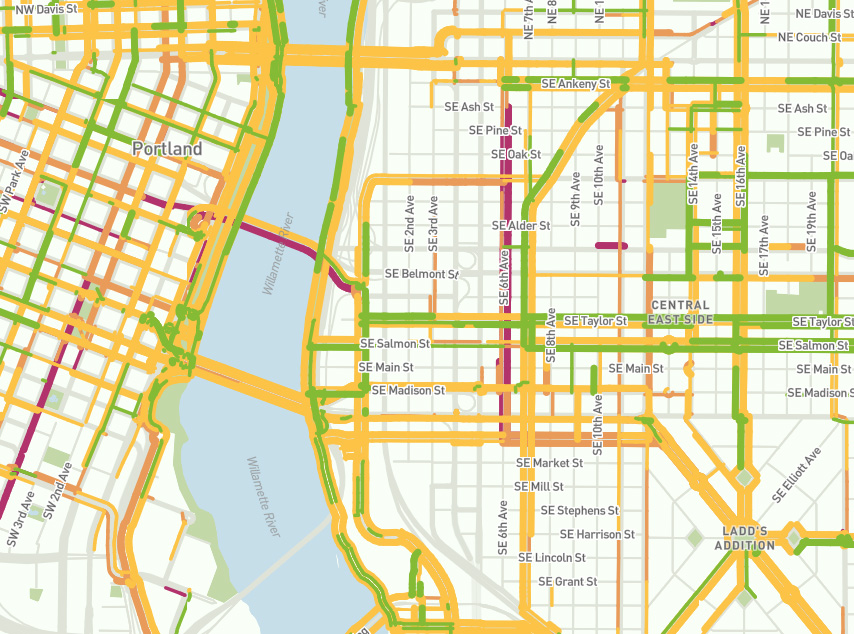
\includegraphics[angle = 0,scale = 0.75]{figure/stress_map.jpg}
  \caption[Ride Report's Stress Map for Portland, OR.]{\normalsize{Ride Report's Stress Map for Portland, OR. Greener road segments incidate less
  stressful streets while more red segments indicate more stressful streets. 
  ``Stress'' is computed by taking the average rating for each segment.}}
  \label{fig:stress-map}
  \end{figure}
  
  The app is designed to minimize barriers to response in order to
  maximize sample size, at the expense of ensuring quality and consistent
  responses. It automates all of the data collection except the rating,
  and the rating only requires (and allows) a binary response. There is no
  direct prompting from the app indicating what criteria cyclists should
  be using to evaluate their rides, other than the labels for the binary
  ratings. In addition, riders' rating their rides on \textit{Ride Report}
  are volunteers, so they are under no obligation to rate their rides. In
  fact, most of the rides lack ratings, and we have no guarantee that the
  pattern of missing ratings is ignorable.
  
  The end goal of collecting and studying this data is to be able to
  accurately map which roads are not serving bicycle commuters well. This
  paper makes steps toward this goal by building models that predict ride
  rating based on information other than route. (We did not create models
  that involve routes, but we do propose ways of modeling routes in
  \autoref{routes}.) The models we discuss, besides measuring the effect
  of weather, time of day, and ride length on the probability of a
  negative rating, address two nontrivial issues in this data: the
  variability in how different riders rate their rides and the problematic
  missing ratings.
  
  We are not the first to worry about the issue of variability in riders
  interpretations of what a good or bad route is. As Meyers, a previous
  researcher examining the \textit{Ride Report} data observed, ``everyone
  has different standards for what a `good' or `bad' ride is, and the data
  might benefit from randomized IDs attached to each cell
  device.''\footnote{Meyers (2015)} Thankfully, \emph{Ride Report} does
  keep track of which rides belong to each to rider. We model the varying
  overall tendencies of each rider to rate a ride negatively with random
  intercepts in a multilevel model. For example, if we let \(y_i\) be the
  rating of the \(i\)th ride and \(X_i\) be the ride-level variables, then
  we can fit a regression:
  
  \[\mathbb{P}(y_i = 1) = \text{logit}^{-1}
  \left( \alpha_{j[i]} +  X_i \beta \right) ,\] where \(\alpha_j\) is an
  intercept specific to rider \(j\). In addition, the rider intercepts
  come from a common distribution,
  \[\alpha_j \sim N (\mu_\alpha, \sigma^2_\alpha),\] where \(\mu_\alpha\)
  is the mean of all the \(\alpha_j\)s. Similar models have been used in
  situations when data consist of subjective ratings, including one study
  examining how people rate sexual attraction\footnote{Mackaronis,
    Strassberg, Cundiff, \& Cann (2013)}.
  
  Missing ratings are another important problem in this data set. While we
  have the route they chose and all associated covariates, the response
  variable (rating) is missing for many rides. As we will discuss in
  \autoref{missing-data}, the pattern of non-response is likely to be
  correlated with the rating the rider would have given, which may mean
  our parameter estimates are inaccurate. To address this problem, we
  implement a version of the expectation maximization algorithm for
  missing data, creating a model that simultaneously estimates the missing
  data mechanism and the ride rating model.
  
  \chapter{Data Sources}\label{data-sources}
  
  We combine several data sources to do our analysis. Information about
  individual rides, including the GPS trace, the rider, and start
  timestamp were provided by Ride Report. Weather data were collected from
  Weather Underground's archive of the KPDX weather station and a Portland
  Fire Bureau station.
  
  Our goal in this chapter is to discuss these data and what
  considerations we should have in mind before exploring it in depth. This
  includes how and by whom the data were collected, who and what this data
  are representative of, and what samples were taken of the data.
  
  Some of these considerations, such as the limited demographics
  represented in the Ride Report data, pose serious limitations to how our
  inferences can be generalized. Others, such as the large number of
  missing responses in the Ride Report data, motivate the analysis we are
  doing in this thesis. Finally, there are other considerations which we
  will acknowledge here, but addressing them is out of the scope of this
  thesis. This data set contains an abundance of potential research
  questions, only a fraction of which could be reasonably addressed in one
  thesis.
  
  \section{Ride Report}\label{ride-report}
  
  Ride Report's data is the focus of this paper. Knock Software created
  the app to collect large amounts of information about urban cyclists'
  routes and experiences on those routes. The hope is that this
  information will be valuable to city planners.\footnote{Knock's other
    project is making a cheaper bicycle counter for cities to monitor
    traffic flow, again intended to be sold to cities wishing to improve
    bike infrastructure.}
  
  Ride Report's approach to crowd sourcing these data is particularly
  important to understand. The app automates every piece of the data
  collection process except for the rating given by the rider. Thus, the
  app casts aside nuanced and (somewhat) reliable human input in favor of
  increasing sample size: one could imagine a similar app where users have
  more control over how the route is recorded, have the ability to rate on
  a more fine-grained scale, and are given more direction in what they are
  rating for. This trade off causes two problems with the reliability with
  the data.
  
  Before we get into the potential issues in the data collection, though,
  let's examine the data collection process itself. When installed on a
  person's phone, the Ride Report app attempts to automatically detect
  when the user starts riding their bicycle, based accelerometer data,
  when a user leaves a familiar Wi-Fi network, and some other pieces of
  information. When the app detects the start of a ride, it starts
  recording a GPS trace. At the end of the users ride, the app detects
  them getting of their bike (in a similar process to how it detected the
  start of a ride) and prompts them to give a rating of the ride. The ride
  data are saved then, even if the user does not provide a rating.
  
  This automatic detection of when a ride starts and stops leads to two
  related and common errors in the dataset: first, one ride is often split
  into two or more rides at points, such as at a stoplight or a train
  crossing, where a cyclist stops for an extended period of time; second,
  car rides are sometimes misclassified as bicycle rides and vice-versa
  (car rides are not rated.) The app allows riders to correct the
  misclassification, but provides no way to join split rides back
  together.
  
  \begin{figure}[tbh]
  \centering
  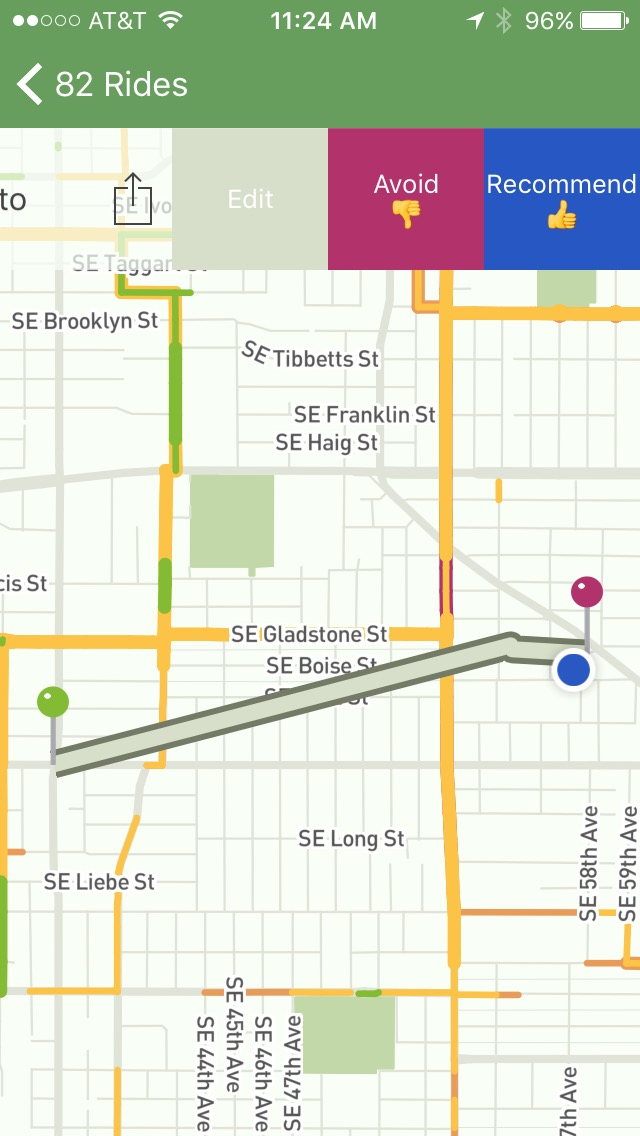
\includegraphics[angle = 0,scale = 0.2]{figure/ride_report_rating.jpg}
  \caption[The Ride Report app's interface]{\normalsize{The Ride Report app's interface has changed significantly between
  versions, including the rating text displayed after a ride. This is the current
  version as of Februrary 2015.}}
  \label{fig:ride-rating}
  \end{figure}
  
  The app only recently became publicly available and has undergone
  significant changes in the course of its life. In particular, while the
  ratings have always been binary, the labels have changed at various
  points in time. At one point the rating labels were ``Stressful'' and
  ``Chill'', while now they are labelled ``Recommend'' and ``Avoid'' (see
  \autoref{fig:ride-rating}). Other fundamentals of the data collection
  process---such as the binary ratings, the automatic collection of GPS
  traces of routes---have remained constant.
  
  The data collection method itself has some problems, but there also may
  be some biases in the population of riders using the app. The app is
  only available on iOS, so only iPhone owners could use this application
  which may imply a bias toward riders of higher socioeconomic status. At
  the time of the start of the thesis, the app was in private beta,
  meaning only people who actively sought out using the app were able to
  use it. Now the application is public and on the Apple App Store, making
  it more widely available. Due to these issues, many of the earlier rides
  may be people within the developer's personal network. Unfortunately,
  it's hard to make any solid conclusions about the users of the app
  because Ride Report doesn't collect any demographic data about their
  riders.
  
  One other issue with the Ride Report data guided our analysis: privacy.
  Because the data involves time stamps and GPS locations of people's
  commutes, the data is very sensitive: one could easily infer someone's
  home and workplace based on their most common routes. In fact, this data
  is protected by an end-user license agreement (EULA) which prevents
  sharing of data, without the explicit permission of those involved. This
  presented a logistical challenge: how were we to do inference and data
  exploration without access to the data?
  
  By agreement with Knock Software, identifying data must be kept private.
  With permission from five riders, Knock was able to give us a small
  subset consisting of all the rides from those five riders, to be kept
  confidential. That is the data set we used for prototyping models and
  some basic exploratory analysis. Knock also agreed to allow us to run
  models fitting scripts on larger samples of their data set, as long as
  they were performed on their computers, with no identifying data leaving
  their system.
  
  While at first this set up seems like an inconvenience, it actually has
  some advantages. One of the pitfalls of having an entire data set,
  especially a high dimensional one, is that in performing exploratory
  analyses it is often too easy to find spurious ``statistically
  significant'' results. Instead, we must come up with our models before
  running them, greatly limiting the choices we can make in the ``garden
  of forking paths.''\footnote{``The garden of forking paths,'' a
    reference to the short story by Jorge Luis Borges, is a term coined by
    Andrew Gelman to refer to the infinite number of choices researchers
    have in analyzing a set of data, which often allows for enough
    flexibility to discover coincidences (``The garden of forking paths,''
    2013).}
  
  \section{Weather Data}\label{weather-data}
  
  Slippery roads and formidable winds are no fun for anyone balancing on a
  two-wheeled vehicle. Weather is, then, one of the most obvious family of
  predictors for ride rating, at least intuitively. We use the time of a
  ride to join in data about the weather conditions during the ride,
  including
  
  \begin{itemize}
  \tightlist
  \item
    the temperature,
  \item
    whether and how much it is raining,
  \item
    whether the roads are wet or have puddles,
  \item
    wind and gust speed.
  \end{itemize}
  
  We include the first two, temperature and precipitation, to account for
  rider comfort. A sweltering, frigid, or stormy day could make an
  unpleasant experience for a bicyclist and thus could lead to more
  negative ratings.
  
  On the other hand, we include the last two, wet road and gust speed, as
  factors that impact safety. During and after storms, puddles often
  accumulate in bike lanes before the center of the road, pushing cyclists
  into lanes shared by cars, which are often more dangerous.
  
  Gust speeds impact the aerodynamics of a ride, which are particular
  important for bicyclists. It's one of the main reasons cyclists care
  about getting into lower (and more aerodynamic) rider positions. Thus,
  high wind or gust speeds may affect rider rating.
  
  \begin{figure}[tbh]
  \centering
  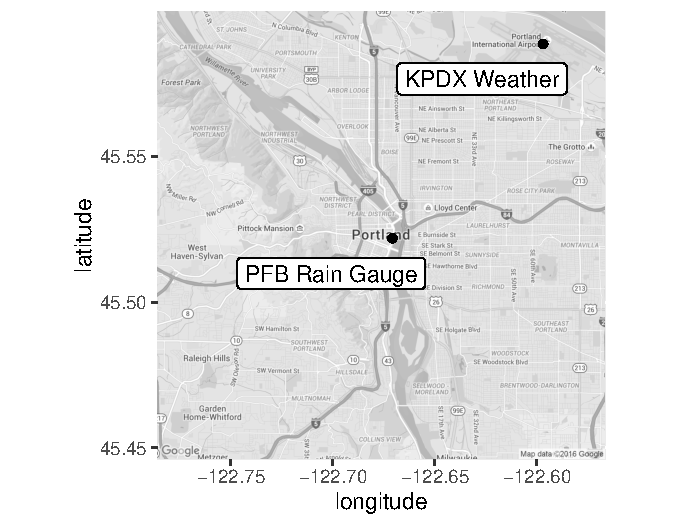
\includegraphics[angle = 0,scale = 1]{figure/weather_station_map.pdf}
  \caption[Locations of weather data collection sites]{\normalsize{Locations of weather data collection sites. Daily weather information
  was collected at the KPDX weather station at Portland International Airport. 
  Hourly precipitation data were collected at the Portland Fire Bureau's rain
  gauge in downtown Portland.}}
  \label{fig:weather-stations}
  \end{figure}
  
  We are limiting our study to rides in Portland, Oregon. Given this, we
  can first assume that it may be reasonable to expect that riders are
  used to the same climate, and thus have somewhat similar responses to
  weather. This also makes it reasonable to use data from one nearby
  weather station, rather than attempting to collect from several stations
  and creating a spatial model for weather.
  
  For daily summaries of weather conditions, we used weather history from
  the KPDX weather station at Portland International Airport downloaded
  from Weather Underground.\footnote{Weather Underground (2016)} From this
  we were able to get daily weather data, including
  
  \begin{itemize}
  \tightlist
  \item
    Average, minimum, maximum temperature for the day.
  \item
    Total precipitation.
  \item
    Mean wind speed, as well as gust speed (speed of brief, strong winds.)
  \end{itemize}
  
  We also got hourly rainfall data from a data stream at the Portland Fire
  Bureau Rain Gage at 55 SW Ash St.,\footnote{Portland Bureau of
    Environmental Science (2016)} which is just about the geographic
  center of Portland. This just gives raw uncorrected rain gauge data, but
  gives us a fine grain look at how much rain there has been recently.
  
  For daily weather data, such as temperature highs and average wind
  speed, we use information from the KPDX weather station. It is further
  from the geographic center of the rides we are examining, but because
  the weather is daily summary statistics, we don't expect closer weather
  stations to be much more informative. \autoref{fig:weather-stations}
  shows the geographic positions of these two stations.
  
  \section{Notation for the Joined Data Set}\label{data-notation}
  
  We combined the ride records with weather data by joining by start date
  stamp of the ride. We will denote our set of ride-level predictors, each
  of which is an \(n\) by 1 column vector as,
  
  \begin{itemize}
  \tightlist
  \item
    \(x^\text{length}\), log ride length, scaled to have mean 0 and
    standard deviation of 1
  \item
    \(x^\text{rain}\), rainfall during hour of ride, in tenths of inches
  \item
    \(x^\text{rain4h}\), rainfall during past four hours before ride, in
    tenths of inches
  \item
    \(x^\text{wind}\), mean wind speed for the day, in miles per hour
  \item
    \(x^\text{gust}\), max gust speed for the day, in miles per
    hour\footnote{Gust speeds are the max speeds of winds that are fast,
      highly variable, and short-term. For METAR weather stations, which
      the KPDX station is, gust speeds report the maximum wind speed when
      there were rapid fluctuations in wind speed with at least 10 knots
      in the difference between the lows and highs.}
  \item
    \(x^\text{temp}\), average temperature, in degrees Fahrenheit for the
    day.
  \end{itemize}
  
  We will often represent this set of predictors as the ride-level
  predictor matrix
  \(X = (x^\text{length} \; x^\text{rain} \; x^\text{rain4h} \; x^\text{wind} \; x^\text{gust}\; x^\text{temp}).\)
  We also have the predictor \(t \in [0, 24]^n\), representing the time of
  day of the ride, measured by hours since midnight. (Because it must be
  modelled in a different fashion than the other variables, we use the
  simple notation of a single letter for it.)
  
  Let \(y_i = 1\) if the \(i\)th ride received a negative rating, and
  \(y_i = 0\) if it received a positive rating, for \(i = 1, \ldots, n\).
  Choice of coding which events are 0's and which are 1's is arbitrary
  when making logistic regression models, though we made this choice
  because for the sake of our analysis, negatively rated rides are more
  interesting events. For urban planning applications, they define the
  areas that need attention.
  
  \chapter{Methods}\label{methods}
  
  We use many statistical methodologies in this paper. We outline here the
  central methods used, both to familiarize the reader and to establish
  the notation we use throughout this paper. The models we present combine
  logistic regression, multilevel\footnote{Multilevel models are often
    referred to as hierarchical models or mixed effects models.} models,
  additive models, and smoothing splines. We also make use of two recently
  developed graphical model evaluation tools: the separation plot and the
  heat map plot.
  
  The one large methodology not covered here is the expectation
  maximization algorithm we use to model the missing data mechanism for
  missing ride ratings. The theory of that algorithm is outlined in
  \autoref{missing-data} and an example of its implementation can be found
  in \autoref{em-implementation}.
  
  \section{Logistic Regression}\label{logistic-regression}
  
  Statistical models are often split into regression models---models with
  a quantitative response---and classification models---models with a
  categorical response. Thus, it may seem odd that we are using a
  regression model when our response variable, ride rating, is a binary
  outcome.
  
  But, when modeling a binary variable \(Y\), we consider it a Bernoulli
  random variable, \[Y \sim \text{Bernoulli}(p),\] where \(p\) is the
  probability the response is 1 and \(1-p\) is the probability the
  response is 0. So our response variable \(Y\) may be binary, but the
  primary quantity of interest behind that outcome is \(p\), a
  quantitative variable. This is why we consider logistic regression a
  regression model.
  
  Logistic regression is one form of a generalized linear model. Recall
  that in linear regression we use data with response variable \(y_i\) and
  \(j\) predictors \(x_{i1}, \ldots, x_{ij}\) to fit the best-fitting
  linear function
  
  \[y_i = \beta_0 + \beta_1 x_{i1} + \cdots + \beta_j x_{ij} + \epsilon,\]
  where \(\epsilon \sim N(0, \sigma^2)\), by estimating
  \(\beta_0, \ldots, \beta_j\). We can equivalently write,
  
  \[y_i \sim N(\beta_0 + \beta_1 x_{i1} + \ldots + \beta_j x_{ij}, \sigma^2).\]
  
  We could, in fact, try to predict \(p\) with a linear regression, though
  such a model will always have the problem of predicting probabilities
  outside of the range of \([0, 1]\). That's not a recipe for simple
  interpretation or reliable predictions. A generalized linear model uses
  a ``link function,'' \(g\), to modify the regression so the range of the
  response more accurately reflects the practical range of the variable;
  i.e.~model:
  
  \[g(y_i) = \beta_0 + \beta_1 x_1 + \ldots + \beta_j x_j + \epsilon_i.\]
  
  In logistic regression, the ``link'' function is the logit function,
  \(\text{logit}:[0,1] \to \mathbb{R}\),
  
  \[\text{logit} (p) = \log \left(\frac{p}{1-p}\right). \]
  
  This function is also known as the log-odds, because odds are defined as
  \(p/1-p\) for any probability \(p\).
  
  So in logistic regression, we model the probability of \(y_i = 1\) as,
  
  \[\mathbb{P} (y_i = 1) = \text{logit}^{-1} (\beta_0 + \beta_1 x_1 + \ldots + \beta_j x_j).\]
  
  Notice that the inverse logit function\footnote{sometimes called the
    logistic function} maps values from \(\mathbb{R}\) to \([0,1]\). Thus,
  the function provides a convenient way to map linear combinations of
  other variables onto values that are valid probabilities. Other such
  functions exist and are also used for regressions with binary responses,
  such as the probit function. Logistic regression, however, is easier to
  interpret---because of the odds connection---and more efficient to
  compute.
  
  \begin{figure}[tbh]
  \centering
  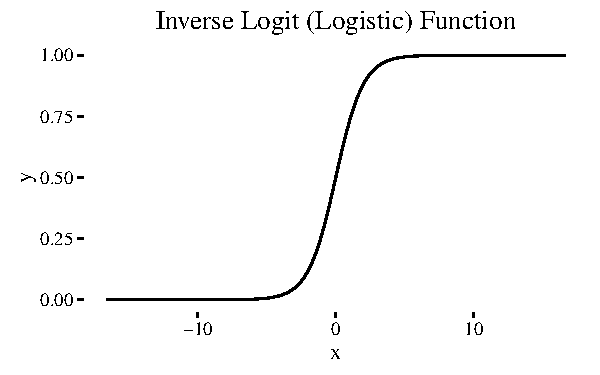
\includegraphics[angle = 0,scale = 1]{figure/logit_plot.pdf}
  \caption[The inverse logit function]{\normalsize{The inverse logit function gives a convenient way to map linear
  combinations of real numbers to valid probability values.}}
  \label{fig:logit-plot}
  \end{figure}
  
  Though coefficients from a logistic regression can't be interpreted the
  same way as a linear model, they do have a convenient interpretation.
  Because the linear part of the model represents log odds, the
  coefficients are log odds ratios; That is, the exponentiated
  coefficients \(e^{\beta_1}, \ldots, e^{\beta_j}\) represent the
  multiplicative effect a one-unit increase in the corresponding predictor
  has on the odds. For example, if we fit a simple logistic regression
  with \(\mathbb{P}(Y = 1) = \text{logit}^{-1} (\alpha + \beta + X)\), we
  could interpret \(e^{\beta} = 1.1\) as meaning that a one unit increase
  in \(X\) gives a 10\% increase in the odds that \(Y = 1\).
  
  \section{Hierarchical Models and Mixed Effects Models}\label{h-models}
  
  Data often contain hierarchies. For example, a set of students' test
  scores may contain the hierarchy of districts and schools those students
  attend. Or a set of soil samples may have been taken at several distinct
  sites, thus having a hierarchy of sites and samples. In the bike ride
  data we examine, there is the hierarchy of riders and rides.
  
  We will talk about different ``levels'' of variables corresponding to
  places in this hierarchy. When we refer to ``ride-level variables,'' we
  refer to variables that are specific to a ride, whereas we refer to
  ``rider-level variables'' as those specific to the rider, and thus also
  all the rides that rider takes. For example, we consider length a
  ride-level variable and total number of rides taken a rider-level
  variable.
  
  We will also discuss road segment-level variables, which are variables
  that are specific to the road segments in the route of a ride
  (e.g.~length, presence of bike lanes, etc). But there isn't a clear road
  segment-ride hierarchy: each ride contains multiple road segments and
  each road segment is contained by multiple rides. Thus, this isn't a
  case where multilevel modeling is applicable. (The ideas behind it,
  though, may be fruitfully adapted, as we discuss in \autoref{routes})
  
  Gelman describes two traditional ways of dealing with hierarchical data
  that multilevel models contrasts with: ``complete pooling'' and ``no
  pooling.''\footnote{Gelman \& Hill (2006), p.~7} In ``complete
  pooling,'' we ignore the group-level variables, and give identical
  estimates for parameters for every group. In ``no pooling,'' we do
  entirely separate regressions for each group. Multilevel models are a
  compromise between these extremes (``partial pooling'', as Gelman calls
  it) where all the data are considered in a single regression with some
  parameters shared between groups and some different between groups.
  
  These multilevel models work for other forms of regression, but we will
  focus on logistic regression, as it is the method we use in this paper.
  We will be using notation adapted from Gelman and Hill's description of
  multilevel models.\footnote{Gelman \& Hill (2006), p.~251--252} Consider
  a data set composed of
  
  \begin{itemize}
  \tightlist
  \item
    \(n\) observations of a binary response variable \(y_i\),
    \(i \in 1, \ldots, n\),
  \item
    \(p\) observation-level predictors \(X_i = x_i^1, \ldots, x_i^p\),
  \item
    \(j\) groups into which the observations are split,
  \item
    \(l\) group-level predictors
    \(U_{j[i]} = u_{j[i]}^1, \ldots, u_{j[i]}^l\), where \(j[i]\) is the
    group of the \(i\)th observation.
  \end{itemize}
  
  We could fit a model where the intercept varies by group:
  
  \begin{equation}
  y_i \sim \text{Bernoulli} \left( \text{logit}^{-1}
  \left( \alpha_{j[i]} + X_i \beta  \right) \right),
  \end{equation}\begin{equation}
  \alpha_{j[i]} \sim N(\gamma_0 + U_{j[i]} \gamma, \sigma_{\alpha}^2),
  \end{equation}
  
  where \(\alpha_{j[i]}\) is the intercept for the \(j\)th group,
  \(\beta\) is a vector of coefficients for the observation-level
  predictors, \(\gamma_0\) are the group-level intercepts, and \(\gamma\)
  is a vector of coefficients for the group-level predictors. We could
  also specify a similar model where there are no group-level predictors,
  such that we simply have different intercepts for each group,
  
  \begin{equation}
  \alpha_{j[i]} \sim N(\gamma_0, \sigma_{\alpha}^2).
  \end{equation}
  
  We can also consider a model that has slopes varying by group. For
  simplicity, let's consider just one observation-level predictor,
  \(x_i\), that will have varying slopes \(\beta_{j[i]}\) as well as one
  group-level predictor, \(u_j\). We could specify the model as,
  
  \begin{equation}
  y_i \sim \text{Bernoulli} \left( 
  \text{logit}^{-1} (\alpha_{j[i]} + \beta_{j[i]} x_i) \right),
  \end{equation}
  
  \begin{equation}
  \left(
  \begin{array}{c}
  \alpha_{j}\\
  \beta_{j}
  \end{array}
  \right) =
  N \left(
  \left(
  \begin{array}{c}
  \gamma_0^\alpha + \gamma_1^\alpha u_j\\
  \gamma_0^\beta + \gamma_1^\beta u_j
  \end{array}
  \right),
  \left(
  \begin{array}{cc}
  \sigma^2_\alpha & \rho \sigma_\alpha \sigma_\beta\\
  \rho \sigma_\alpha \sigma_\beta & \sigma^2_\beta
  \end{array}
  \right)
  \right).
  \end{equation}
  
  These models can be fit with maximum likelihood estimation using the
  \texttt{lme4} package in \textit{R}(Bates, Mächler, Bolker, \& Walker,
  2015) or can be fit with Bayesian MCMC using \textit{Stan}(Carpenter et
  al., 2016). The latter has the advantage of making it easy to estimate
  group-level uncertainty at the expense of more computation. We fit
  models using \texttt{lme4}, but make use of \textit{Stan} when we have
  ride-level parameters we want to estimate, in \autoref{stan-model}.
  
  \section{Additive Models and Smoothing
  Splines}\label{additive-models-and-smoothing-splines}
  
  Often, it is helpful to allow more flexibility in the functional forms
  in the models. While parametric models, like logistic regression, assume
  a particular form for the relationship between the variables and
  response, nonparametric models use the data to determine both the
  functional form and values of the parameters in models. However, the
  curse of dimensionality (the more predictors that are in a model, the
  fewer similar observations there are to any observation) can impair
  nonparametric models. Additive models, however, are able to keep a lot
  of the flexibility of nonparametric methods while avoiding the curse of
  dimensionality. Additive models assume that the response is the sum of
  functions of each of the predictors:
  
  \[\text{logit} (\mathbb{P}(y_i = 1)) =
  \alpha + \sum_{j = 1}^p f_j(x_{ij}).\]
  
  These functions can be linear, so generalized linear regression is a
  subset of additive models. But more interestingly, these functions can
  be non-parametric.\footnote{How are these models fit? Using what's known
    as the Backfitting Algorithm. We define the \(k\)th partial residuals
    \(Y^{(k)} = Y - \left(\alpha + \sum_{j \neq k} f_j(x_j)\right)\).
    (That is, define the portion of \(Y\) leftover for \(f_k(x_k)\) to fit
    to after the other \(f_j\)'s have had their share.) Then, iteratively
    fit each of the functions \(f_j\) on the partial residuals \(Y^{(j)}\)
    until each of the functions converge. For a further quick look at
    additive models, check out Cosma Shalizi's lecture notes (Shalizi
    (2013a))} One of the most common types of functions fit are smoothing
  splines.
  
  Smoothing splines are essentially cubic functions stitched together at
  points called ``knots'' such that the full piece-wise function is
  continuous and has continuous first and second derivatives. One can
  further define cyclic cubic splines, which simply have the constraint
  that the last knot and first knot be treated as the same knot, thus
  allowing a continuous cyclic function to be fit.\footnote{For a brief
    and entertaining introduction to smoothing splines, see Shalizi
    (2013b). For a more in-depth look at splines, check out Wood (2006)}
  
  Computation of multilevel additive models with splines is available in
  the \texttt{gamm4} package (Wood \& Scheipl, 2014).
  
  \section{Tools for Evaluating Models}\label{evaluate}
  
  After fitting our models, we will want to know how each of our models
  compare. Did adding a particular term enhance or diminish the accuracy
  of our model? Instead of focusing on one measure of fit we use several.
  Log likelihood and AIC provide useful summaries of fits to the data
  based on the likelihood function. Separation plots---which we discuss in
  the next section---allow us to assess the predictive ability of a model;
  in particular, can the model identify high and low probability events?
  We also use the area under the ROC curve (AUC) measure popular for
  assessing logistic regression. In particular, we compute 10-fold cross
  validated ROC statistics to detect if models are overfitting to the
  data.
  
  \subsection{The Separation Plot}\label{the-separation-plot}
  
  The separation plot, created by Greenhill, Ward, and Sacks\footnote{Greenhill,
    Ward, \& Sacks (2011)}, is designed to show how well a logistic
  regression model can distinguish between high and low probability
  events.
  
  \begin{figure}[tbh]
  \centering
  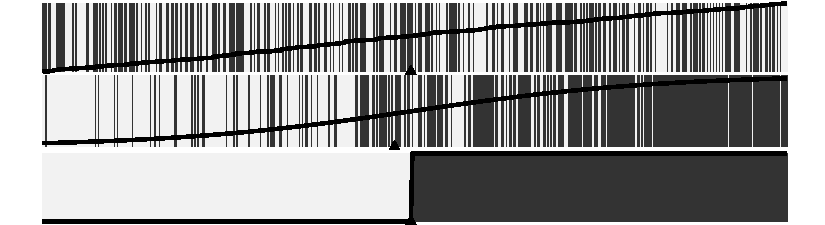
\includegraphics[angle = 0,scale = 1]{figure/sep_plot_examples.pdf}
  \caption[Examples of three separation plots]{\normalsize{Examples of three separation plots. The first plot shows
  what it looks like when $y$ and $\hat{y}$ are uncorrelated. The second plot 
  shows a fairly good model, where the $y$ are generated as Bernoulli($\hat{y}$).
  The third plot shows a model where the responses are fully separated.}}
  \label{fig:sep-plot-examples}
  \end{figure}
  
  Let \(y\) be a vector of observed binary response and \(\hat{y}\) a
  vector of predicted probabilities of a 1 for each observation, predicted
  by some model. Then we can construct the plot as follows: We plot the
  data \((y, \hat{y})\) as a sequence of vertical stripes, colored
  according to observed outcome, \(y\), and ordered from low to high
  probability based on \(\hat{y}\). A curve is superimposed upon the
  stripes showing the \(\hat{y}\) as a line graph. And finally, a small
  triangle is placed indicated the point at which the two colors of lines
  would meet if all observations \(y = 0\) were placed to the left of all
  the \(y=1\) observations; \textit{i.e.} showing where the boundary would
  be if the two classes were perfectly separated by the model.
  
  Separation plots don't do well with larger sample sizes: if there are
  too many observations, it becomes difficult to read. There are several
  ways around this, but we choose to randomly sample the observations.
  
  \chapter{Modeling Rides and Riders}\label{model-chapter}
  
  Complex statistical models can accurately model intricate processes. But
  they also run the risk of overfitting to the data. To avoid this, we
  build up our models from simple to complex, comparing the models with
  cross validation to make sure the complexities introduced add real
  value.
  
  In this chapter we focus on building models that incorporate information
  about rider, weather conditions, time of day, and ride length. In brief,
  our models start with a logistic regression model considering only
  ride-level variables, and formulate more complex models by adding
  various terms. \autoref{tab:models} describes each model briefly along
  with the models label.
  
  \begin{longtable}[]{@{}ll@{}}
  \caption{Brief descriptions of Models 1--6
  \label{tab:models}}\tabularnewline
  \toprule
  \begin{minipage}[b]{0.13\columnwidth}\raggedright\strut
  \textbf{Model}
  \strut\end{minipage} &
  \begin{minipage}[b]{0.72\columnwidth}\raggedright\strut
  \textbf{Description}
  \strut\end{minipage}\tabularnewline
  \midrule
  \endfirsthead
  \toprule
  \begin{minipage}[b]{0.13\columnwidth}\raggedright\strut
  \textbf{Model}
  \strut\end{minipage} &
  \begin{minipage}[b]{0.72\columnwidth}\raggedright\strut
  \textbf{Description}
  \strut\end{minipage}\tabularnewline
  \midrule
  \endhead
  \begin{minipage}[t]{0.13\columnwidth}\raggedright\strut
  Model 1
  \strut\end{minipage} &
  \begin{minipage}[t]{0.72\columnwidth}\raggedright\strut
  (Baseline) logistic regression
  \strut\end{minipage}\tabularnewline
  \begin{minipage}[t]{0.13\columnwidth}\raggedright\strut
  Model 2
  \strut\end{minipage} &
  \begin{minipage}[t]{0.72\columnwidth}\raggedright\strut
  Add rider intercepts
  \strut\end{minipage}\tabularnewline
  \begin{minipage}[t]{0.13\columnwidth}\raggedright\strut
  Model 3
  \strut\end{minipage} &
  \begin{minipage}[t]{0.72\columnwidth}\raggedright\strut
  Add trigonometric terms for time of day
  \strut\end{minipage}\tabularnewline
  \begin{minipage}[t]{0.13\columnwidth}\raggedright\strut
  Model 4
  \strut\end{minipage} &
  \begin{minipage}[t]{0.72\columnwidth}\raggedright\strut
  Additive model with cubic cyclic spline for time of day
  \strut\end{minipage}\tabularnewline
  \begin{minipage}[t]{0.13\columnwidth}\raggedright\strut
  Model 5
  \strut\end{minipage} &
  \begin{minipage}[t]{0.72\columnwidth}\raggedright\strut
  Additive model with spline for ride length
  \strut\end{minipage}\tabularnewline
  \begin{minipage}[t]{0.13\columnwidth}\raggedright\strut
  Model 6
  \strut\end{minipage} &
  \begin{minipage}[t]{0.72\columnwidth}\raggedright\strut
  Remove random rider intercepts from Model 4
  \strut\end{minipage}\tabularnewline
  \bottomrule
  \end{longtable}
  
  \section{Six Models for Probability of a Negative Ride
  Rating}\label{ride-models}
  
  \textbf{Model 1}, which we will use as the baseline for comparing
  further models, is a logistic regression model:
  
  \[ \mathbb{P} (Y_i=1) = \text{logit}^{-1} (\alpha + X_i \beta),\] where
  \(\alpha \in \mathbb{R}\) and \(\beta \in \mathbb{R}^p\) are parameters
  to be estimated. (\(X\) is the matrix of ride-level predictors specified
  at the end of \autoref{data-notation}.)
  
  \begin{figure}[tbh]
  \centering
  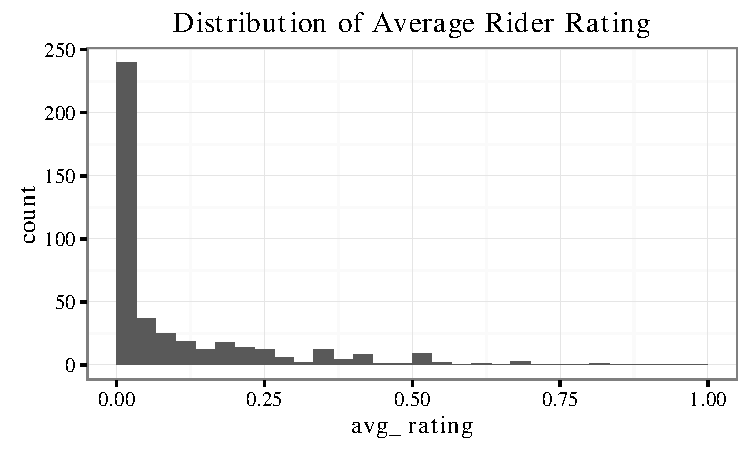
\includegraphics[angle = 0,scale = 1]{figure/rider_avgs.pdf}
  \caption[Distribution of Average Rider Rating]{\normalsize{The overall rates at which each rider gives a negative rating for a
  ride varies greatly. This is our primary motivation for including rider intercepts
  and predictors.}}
  \label{fig:rider-avgs}
  \end{figure}
  
  Riders appear to have different tendencies to rate rides negatively more
  often, as we note in \autoref{fig:rider-avgs}. In fact, many riders give
  zero or nearly zero negative ratings. For \textbf{Model 2}, we account
  for this variability by adding intercepts that vary by rider:
  
  \begin{equation}
  y_i \sim \text{Bernoulli} \left(
  \text{logit}^{-1} \left( \alpha + \alpha_{j[i]} + X_i \beta \right)
  \right),
  \end{equation}
  
  for \(i = 1, \ldots, n\).
  
  Rider intercepts themselves aren't as interesting as how they deviate
  from the mean, so we keep a fixed intercept \(\alpha\) and constrain the
  rider intercepts, \(\alpha_j\), by specifying
  
  \[\alpha_j \sim N(0, \sigma^2_\alpha).\]
  
  Starting with \textbf{Model 3}, we address time of day,
  \(t \in [0, 24)\) as a predictor. (We measure time of day in hours since
  midnight.) We use time of day to account for all the daily trends that
  may affect ratings, including as a simple way to model the overall
  traffic level, which is difficult to model on its own. These patterns
  are cyclic and very non-linear, so we can't model time as a linear term.
  One approach is to add sinusoidal terms with a period of one day. We
  would be interested in fitting a term,
  
  \[\beta \sin (T x^{\text{time}} + \phi).\]
  
  Estimating \(\beta\) wouldn't be hard: we can easily estimate
  coefficents of transformed terms; it's more difficult to estimate \(T\)
  and \(\phi\). But, we know that we want to restrict our terms to fitting
  trends that happen over the course of one day, so we can set
  \(T = 2 \pi / d\), where \(d\) is 24 hours or some fraction of that.
  
  As for \(\phi\), a trigonometric transformation reframes the estimation
  of a phase shift parameter into the estimation of two coefficients for
  trigonometric functions with no phase shift:
  
  \begin{align*}
  \beta \sin (T x + \phi) &= 
  \beta \left( \sin (T x) \cos (\phi) + \cos (T x) \sin (\phi) \right)\\
  &= \beta \cos (\phi)) \sin (T x) + \sin (\phi) \cos (T x)\\
  &= \beta_1 \sin (T x) + \beta_2 \cos (T x),
  \end{align*}
  
  where \(\beta_1 = \beta \cos (\phi)\) and \(\beta_2 = \sin (\phi).\) At
  this point, we are now just estimating the coefficients of a couple of
  transformed variables, which can easily be done in any package that does
  generalized linear regressions.
  
  We also want to take into account that weekday hourly patterns may be
  different than weekend patterns. We use a variable \(X^\text{weekend}\)
  that serves as a weekend indicator. For Model 3, we add two sets of
  sinusoidal terms: one set for weekdays and one for weekends. More
  explicitly, we define the model,
  
  \begin{equation}
  \begin{split}
  \mathbb{P} (Y_i=1) = \text{logit}^{-1} (&\alpha + \alpha_{j[i]} + X_i \beta \\
  &+ X^\text{weekend} \cdot [\beta^{t1} \sin(T \cdot t) + \beta^{t2} \cos (T \cdot t)\\
  &+ \beta^{t3} \sin(T/2 \cdot t) + \beta^{t4} \cos (T/2 \cdot t)]\\
  &+ (1 - X^\text{weekend}) \cdot [\beta^{t1} \sin(T \cdot t) + \beta^{t2} \cos (T \cdot t)\\
  &+ \beta^{t3} \sin(T/2 \cdot t) + \beta^{t4} \cos (T/2 \cdot t))].
  \end{split}
  \end{equation}
  
  For \textbf{Model 4} we abandon parametric methods and use a cyclic
  non-parametric smoother to model time of day, making our model,
  
  \begin{equation}
  y_i \sim \text{Bernoulli} \left(
  \text{logit}^{-1} \left( \alpha + \alpha_{j[i]} + X_i \beta + 
  X^\text{weekend} \cdot f^\text{time.w} (t_i) +
  (1 - X^\text{weekend}) \cdot f^\text{time} (t_i) \right)
  \right),
  \end{equation}
  
  for \(i = 1, \ldots, n\), where \(\alpha_j\) is specified like Model 2
  and \(f^\text{time.w}\) and \(f^\text{time}\) are cyclic cubic spline
  terms for weekend and weekday rides, respectively, with knots at 0, 3,
  6, 9, 12, 15, 18, 21, and 24 (0, again) hours.
  
  \textbf{Model 5} extends Model 4 by adding a cubic spline for
  ride\_length:
  
  \begin{equation}
  y_i \sim \text{Bernoulli} \left(
  \text{logit}^{-1} \left( \begin{split} 
  &\alpha + \alpha_{j[i]} + X_i \beta + 
  f^\text{length} (x^\text{log.length}_i) +\\
  &X^\text{weekend} \cdot f^\text{time.w} (t_i) +
  (1 - X^\text{weekend}) \cdot f^\text{time} (t_i)
  \end{split}
  \right)
  \right),
  \end{equation}
  
  for \(i = 1, \ldots, n\), where \(f^\text{length}\) is a cubic spline
  smoother.
  
  Finally, \textbf{Model 6} is identical to Model 5, but without the rider
  intercepts:
  
  \begin{equation}
  y_i \sim \text{Bernoulli} \left(
  \text{logit}^{-1} \left( \alpha + X_i \beta + 
  f^\text{time} (t_i)  \right)
  \right),
  \end{equation}
  
  for \(i = 1, \ldots, n\), where \(f^\text{time}\) is a cyclic cubic
  spline term, with the same knots as in Model 4.
  
  \section{Model Evaluation}\label{model-evaluation}
  
  \begin{table}[htb]
  \centering
  \caption{Fit summaries for Models 1--6.\label{tab:modelfits}}
  \begin{tabular}{lm{4in}rrr}
  \toprule
  \textbf{Model} & \textbf{Separation Plot} & \textbf{$\log (\mathcal{L})$} & \textbf{AIC} &
  \textbf{AUC}$_{\text{CV}}$\footnotemark\\
  \midrule
  Model 1 & 
\includegraphics{figure/model1-sep.pdf}
  & -4,786 & 9,586 & 0.552\\
  Model 2 & 
\includegraphics{figure/model2-sep.pdf}
  & -3,971 & 7,957 & 0.797\\
  Model 3 & 
\includegraphics{figure/model3-sep.pdf}
  & -3,923 & 7,877 & 0.802\\
  Model 4 & 
\includegraphics{figure/model4-sep.pdf}
  & -3,930 & 7,870 & 0.802\\
  Model 5 & 
\includegraphics{figure/model5-sep.pdf}
  & -3,928 & 7,878 & 0.803\\
  Model 6 & 
\includegraphics{figure/model6-sep.pdf}
  & -4,713 & 9,455 & 0.601\\
  \bottomrule
  \end{tabular}
  \end{table}
  
  \footnotetext{Area under ROC curve estimated with  10-fold cross-validation.}
  
  To fit the data, we got all of the rides in Portland, OR, from December
  3, 2014 to February 8, 2016 for riders that had over 20 rated rides. (We
  only look at riders with a certain number of rides to make sure we get
  can get estimates for rider-level parameters, like rider random
  intercepts, that aren't too uncertain.) There were 25,397 rides, 14,032
  of which were rated. Overall, 10.88 percent of these rides were given a
  negative rating. There were 138 riders in the data set.
  
  The separation plots in \autoref{tab:modelfits} give a clear initial
  picture of how these model fits compare. Model 1 performs very poorly
  compared to those that include rider intercepts, assigning the same
  probability to most observations. Models that include the rider
  intercept perform similarly to each other. The log likelihoods and
  AIC,\footnote{Akaike Information Criterion (AIC) is a metric that
    penalizes the \(\log (\mathcal{L})\) with the number of parameters
    estimated \(k\), with lower values being better. It is defined as
    \(\text{AIC} = 2k - 2 \log(\mathcal{L})\).} shown in
  \autoref{tab:modelfits}, corroborate this. Adding time dependency
  doesn't seem to impact predictive ability. We will see later, however,
  that it gives a fascinating result to interpret.
  
  The gains from the rider intercepts are great, but we are compelled to
  ask: how much of that gain could have been achieved with randomly chosen
  groups? In other words, if riders were randomly assigned to rides, would
  the flexibility in the model created by allowing intercepts to vary
  increase predictive performance to the same degree? To test this, we ran
  a Model 4 after we randomly assign the rides a rider, by randomly
  permuting the rider column. This quick test nullified this skepticism,
  as you can see in the resulting separation plots in
  \autoref{fig:sep-plots-intercept-test}.
  
  \begin{figure}[tbh]
  \centering
  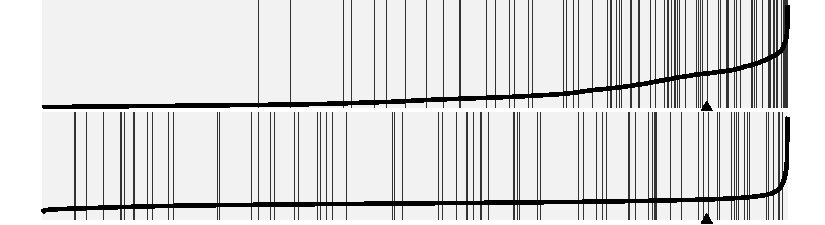
\includegraphics[angle = 0,scale = 1]{figure/intercept_test_plot.pdf}
  \caption[Separation plots for models 2 compared to a similar model where
  riders are randomly assigned to rides]{\normalsize{Separation plots for models 2 compared to a similar model where
  riders are randomly assigned to rides. This test demonstrates that the 
  improvement in predictive performance provided by the rider intercepts
  was not coincidence.}}
  \label{fig:sep-plots-intercept-test}
  \end{figure}
  
  \section{Model Results}\label{model-results}
  
  \begin{table}[htb]
  \centering
  \def\arraystretch{1.3}
  \caption[Regression coefficients for Models 1, 2, 4, and 6.]{Regression coefficients for Model 1, Model 2, Model 4, and Model 6. 
  95\% confidence intervals are given in parentheses.\label{tab:modelcoef}}
  \begin{tabular}{lllll}
  \toprule
   Regression Term &  Model 1 &  Model 2 &  Model 4 & Model 6\\
  \midrule
  Log(length) & -0.122 & -0.100 & -0.092 & -0.114\\
  & \footnotesize (-0.180, -0.063) & \footnotesize (-0.168, -0.032) & 
  \footnotesize (-0.162, -0.022) & \footnotesize (-0.174, -0.054)\\
  Mean Temp. & 0.053 &  0.076 & 0.075 & 0.069\\
  & \footnotesize (-0.0004, 0.110) & \footnotesize (0.005, 0.147) & 
  \footnotesize (0.003, 0.147)  & \footnotesize (0.012, 0.127)\\
  Mean Wind speed & 0.028 & 0.014 & 0.012 & 0.027\\
  & \footnotesize (0.004, 0.052) & \footnotesize (-0.013, 0.041) & 
  \footnotesize (-0.014, 0.039) & \footnotesize (0.002, 0.051)\\
  Gust speed & -0.003 & 0.001 & 0.001 & -0.003\\
  & \footnotesize (-0.015, 0.008) & \footnotesize (-0.012, 0.013) & 
  \footnotesize (-0.012, 0.013) & \footnotesize (-0.014, 0.009)\\
  Rainfall & 0.008 & 0.012 & 0.008 & 0.005\\
  & \footnotesize (-0.015, 0.031) & \footnotesize (-0.015, 0.038) & 
  \footnotesize (-0.019, 0.035) & \footnotesize (-0.019, 0.027)\\
  Rainfall 4-Hour & 0.013 & 0.016 & 0.017 & 0.014\\
  & \footnotesize (0.005, 0.021) & \footnotesize (0.007, 0.025) &
  \footnotesize (0.008, 0.027) & \footnotesize (0.006, 0.022)\\
  Intercept & -2.2868 & -3.075 & -3.127 & -2.313\\
  & \footnotesize (-2.428, -2.108) & \footnotesize (-3.386, -2.764) &
  \footnotesize (-3.436, -2.818) & \footnotesize (-2.475, -2.151)\\ 
  \bottomrule
  \end{tabular}
  \end{table}
  
  \autoref{tab:modelcoef} presents the fixed effect estimates for our
  models. Length has a robust strong negative effect. This makes sense if
  we think of length as the only information we have about route in these
  models: it seems routes that are longer tend to be less likely to be
  rated negatively. Perhaps longer rides tend to be for leisure or sport
  rather than commuting, so and so are less likely to go along routes with
  high traffic and other dangers. Temperature also seems to have a small
  effect. It could be the case that the temperature itself is important,
  or perhaps season is a confounding factor. It could be the case that the
  type of rides taken during the warmer months are more likely to be rated
  negatively. Wind and gust speed don't seem to have robust effects. These
  models suggest that four hour cumulative rainfall was more important
  than rainfall during the hour of the ride. This supports our suspicion
  that weather effects that are more relevant to safety than comfort---
  like wet road and puddles rather than rain at the time of a ride---are
  important in determining a cyclist's rating of their ride. These
  coefficients, however, aren't nearly as enlightening as the time of day
  fits.
  
  \begin{figure}[htb]
  \centering
  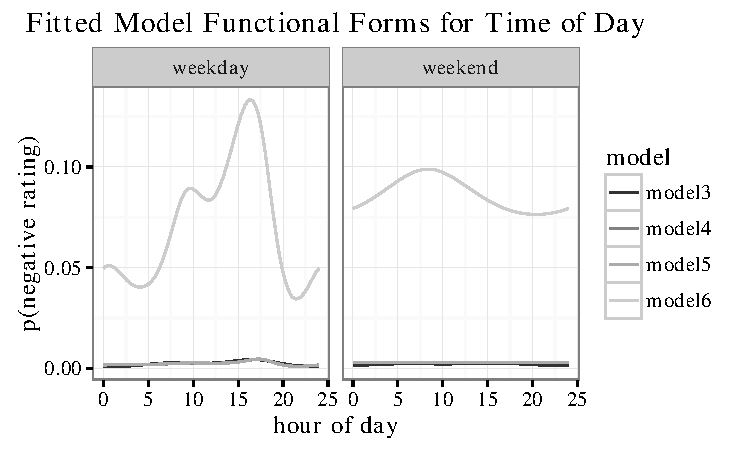
\includegraphics{figure/time_fit_plot.pdf}
  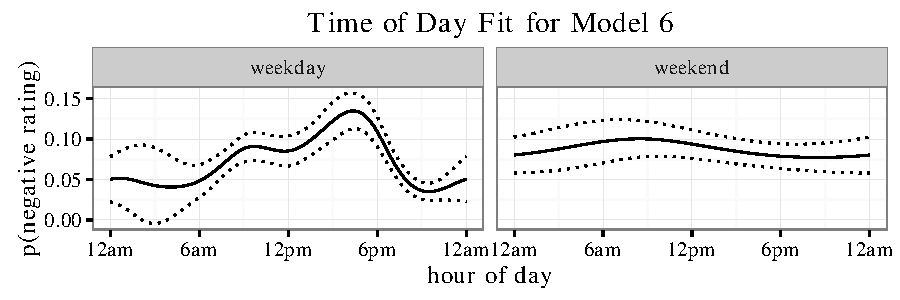
\includegraphics{figure/time_fit_plot_6.pdf}
  \caption[Predicted probabilities of a negative rating by time for a typical ride]{
  Predicted probabilities of a negative rating by time for a typical ride.
  The rider was chosen so the intercept was closest to the mean intercept for model
  5. The median length and average mean temperature were used, and all other
  predictors were set to zero. The dotted lines show $\pm 2$ standard errors from
  the predictions.\label{fig:model-time-fit}}
  \end{figure}
  
  The marginal fits for time of day, shown in
  \autoref{fig:model-time-fit}, are predictable. On weekdays, the
  probability of a negative rating peaks in the afternoon from 4--6 p.m.,
  around when we expect rush hour traffic, and on weekends it stays steady
  throughout the day. While Model 4 and Model 5 give similar fits for time
  of day, Model 3's predictions peak at different times on weekdays and
  exhibit much more variability on weekends. There are two probable
  reasons for these differences: first, the sinusoidal terms are less
  flexible than the splines; second, the splines, because they are
  non-parametric functions, penalize complexity of the fit while the
  parametric sinusoidal form does not, making the splines more
  conservative in their ``curviness.'' The former explains the
  discrepancies in the weekday fits while the latter explains the
  discrepancies in the weekend fits. Given these differences, fitting time
  of day with splines is preferable; there is no motivation to constrain
  the functional form to any strict parametric form.
  
  But these marginal time-of-day fits don't just tell a story about our
  time terms; they also reveal part of why the random rider intercepts are
  such powerful predictors. Notice that in comparing Model 6 to the other
  models in \autoref{fig:model-time-fit}, the scale at which the Model 6
  time fitted probabilities vary is much larger than the scale at which
  the other models' predictions vary. Without allowing for varying rider
  intercepts, the time terms take on a significant role. Yet,
  interestingly, the time term has nowhere near the amount of information
  that the rider intercepts seem to encode, according to the separation
  plots in \autoref{tab:modelfits}.
  
  \begin{figure}[tbh]
  \centering
  \includegraphics[angle = 0,scale = 1]{figure/time_pred_plot.pdf}
  \caption[Predicted probabilities of negative rating by time of day for Models 3--6]{\normalsize{Predicted probabilities of negative rating by time of day for Models 3--6.
  Notice how starting with Model 2, daily trends start to emerge. This indicates that the
  rider intercepts are picking up on time of day trends, which must be reflected in a rider's
  typical ride.}}
  \label{fig:time-pred-plot}
  \end{figure}
  
  \autoref{fig:time-pred-plot} paints a clearer picture of what is going
  on. These models show two different ways to look at the time of day
  pattern in ride rating: Model 2 suggests \emph{who is riding} determines
  these patterns while Model 6 suggests there is something inherent in
  that time of day, such as traffic, that determines these patterns. The
  models between fit a combination of these, but as we saw in
  \autoref{fig:model-time-fit}, the time dependence is more than an order
  of magnitude weaker after accounting for the rider intercepts. The two
  black pillars of rides in the predictions of Models 2--5 line up with
  when we expect commuters to be riding, suggesting that that the riders
  with high rider intercepts are commuters. The converse, however, is not
  true: a great number of rides during commuting times are predicted to
  have almost zero probability of receiving a negative rating.
  
  What explains this relationship between the temporal patterns and the
  rider intercepts? We suspect ride route is a confouding factor here.
  \autoref{fig:time-pred-plot} confirms our suspicion that riders have
  particular schedules they stick to; so it's also likely, given that
  these are mostly commuting cyclists, that most of their rides follow the
  same route as well. These models ignore ride route, so we suspect the
  typical ride route is encoded in the rider intercepts; \emph{i.e.} a
  rider whose commuting route goes through many of the most stressful
  intersections and streets in Portland will likely have a higher
  intercept than most riders. This hypothesis can only be tested, however,
  when future research develops models with random rider intercepts and a
  model for how routes effect ratings.
  
  \chapter{Characterizing Riders}\label{characterizing-riders}
  
  Given the results from last chapter, there is a clear need to understand
  what kinds of riders are in this data set. To do that, we identify
  predictors that differentiate riders and then use these variables to
  identify clusters of riders. We assess how these predictors do as
  rider-level predictors for the rider intercepts.
  
  We also compare random intercepts with riders to random intercept models
  done by cluster. Ride Report, because they need to respect the privacy
  of their users, cannot identify individual riders in the data they
  provide to clients, yet our model results show that differentiating
  riders is crucial to getting good estimates in our models. If we can
  identify clusters of riders in the data set that give us nearly the same
  information as grouping by individuals did, these could be provided by
  Ride Report without the same level of risks to user privacy as
  identifying individual riders.
  
  \section{Extracting Features and Determining
  Clusters}\label{extracting-features-and-determining-clusters}
  
  We characterized riders based on their rides because \emph{Ride Report}
  does not collect data about their users besides their rides and email
  address. We limited our exploration to riders that had over 20 rated
  rides, in order to focus on riders who had been using the app for some
  time and had an identifiable pattern of rides.
  
  Cyclists' patterns in their rides are complex, particularly their time
  patterns. Computing their mean ride length for weekends was useful, but
  mean time of day for their rides does not capture anything meaningful.
  So we took care in selecting features that distinguished different rider
  patterns we saw when exploring the data.
  
  \begin{figure}[htb]
  \centering
  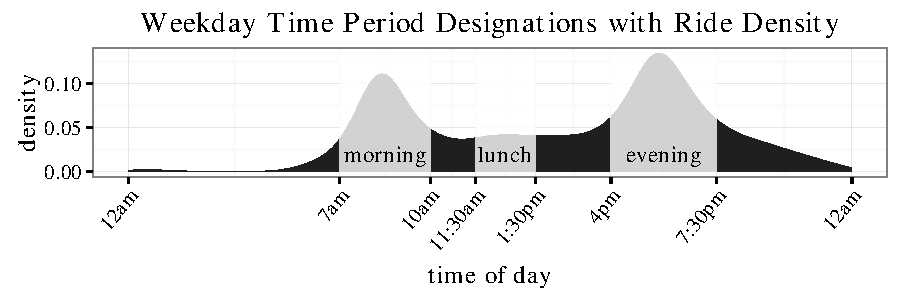
\includegraphics{figure/time-designations.pdf}
  \caption[Time intervals used for morning, lunchtime, and evening in rider feature
  extraction]{Time intervals used for morning, lunchtime, and evening in rider feature
  extraction. These intervals define the time designations we used in clustering. 
  The proportion of each riders rides in each of these time intervals made up three
  of our features.\label{fig:time-splits}}
  \end{figure}
  
  We define the following for each rider \(j\): frequency of
  rides\footnote{We define frequency of a cyclist's rides as the number of
    rides divided by the difference between the time of the most recent
    ride and time of the first ride. (Units are arbitrary, because we
    standardized all of our rider-level variables.)}
  (\(u^\text{freq}_j\)), proportion of rides on weekdays
  (\(u^\text{weekend}_j\)), median length of rides on weekdays
  (\(u^\text{med.len}_j\)) and weekends (\(u^\text{med.len.w}_j\)),
  variance of ride length on weekdays (\(u^\text{var.len}_j\)) and
  weekends (\(u^\text{var.len.w}_j\)), and proportion of weekday rides
  during morning rush (\(u^\text{morning}_j\)), lunch rush
  (\(u^\text{lunch}_j\)), and evening rush (\(u^\text{evening}_j\)). The
  time intervals that describe the morning, lunch, and evening rush are
  shown in \autoref{fig:time-splits}.
  
  \begin{figure}[tbh]
  \centering
  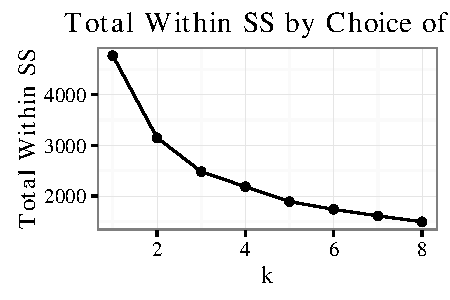
\includegraphics[angle = 0,scale = 0.8]{figure/choice_k.pdf}
  \caption[Comparing total within sum of squares for different $k$ for $k$-means clustering of riders]{\normalsize{Comparing total within sum of squares for different $k$ for $k$-means clustering of riders.}}
  \label{fig:choosing_k}
  \end{figure}
  
  Selecting variables for a cluster analysis is difficult, for the reason
  that many choices about what to use are arbitrary. We have chosen these
  variables, but two important other choices remain: what scales and
  transformations should these variables have? We chose here to transform
  all variables to be approximately gaussian---eliminating the right skew
  that was present in most of these features with log and square root
  transformations---and standardizing them by subtracting their mean and
  dividing by their standard deviation. When clustering, the scaling of
  variables determines how much weight each of them has in determining the
  clusters. Future research may find more appropriate ways to select
  features for clustering, but in our approach here we stick to a naive
  and simple approach to see what we can learn.
  
  \begin{figure}[htb]
  \centering
  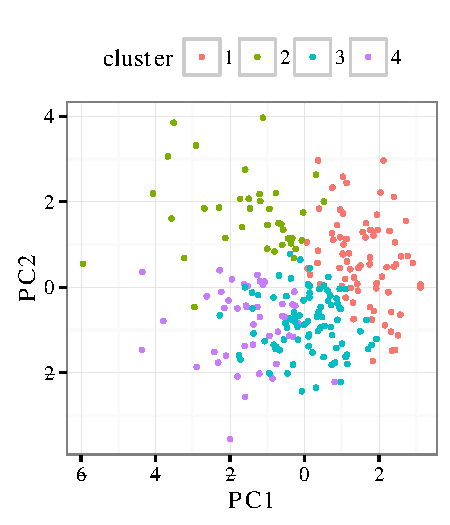
\includegraphics[width=.5\textwidth]{figure/cluster_scatter1.pdf}\hfill
  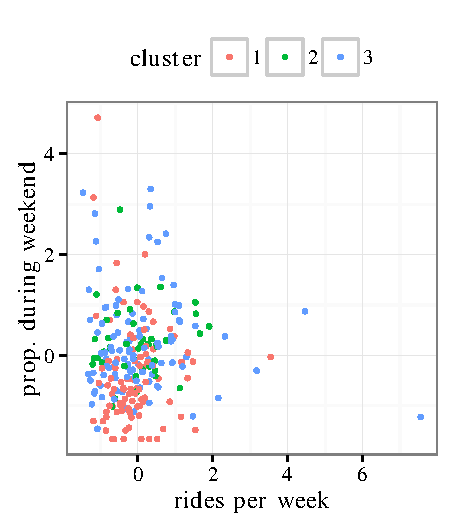
\includegraphics[width=.5\textwidth]{figure/cluster_scatter3.pdf}
  \caption[Rider clusters identified by $k$-means clustering]{
  Rider clusters identified by $k$-means clustering. The triangles represent
  the centroids (computed as the mean) of the cluster members. \label{fig:cluster-scatter}}
  \end{figure}
  
  With the rider-level predictors in hand, we clustered the riders using
  \(k\)-means clustering, which groups a set of points into the \(k\)
  clusters that minimize the within-cluster sum of squared distance to the
  cluster centroids.\footnote{\(k\)-means clustering is fit using a
    hueristic algorithm, which assigns points random to clusters, and then
    repeatedly recomputes the cluster centroids and reassigns the points
    to the cluster with the nearest centroid, until the clusters stop
    changing. This algorithm is fast, but the result is sensitive to the
    initial random assignment, so it is run many times. See page 460 of
    Hastie, Tibshirani, \& Friedman (2008) for more details of \(k\)-means
    clustering.} To choose the number of clusters, we assessed the total
  of the sum of squares within each cluster for different values of \(k\),
  shown in \autoref{fig:choosing_k}, and selected \(k = 4\) as the point
  where we thought after which there was little value in having more
  clusters.
  
  \begin{figure}[bht]
  \centering
  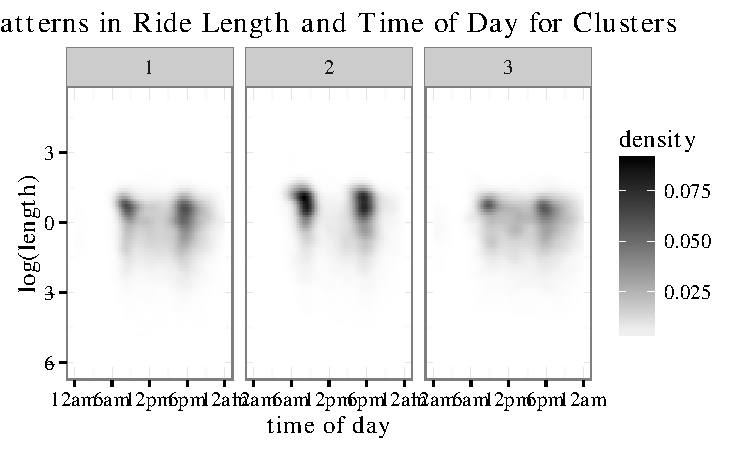
\includegraphics[angle = 0,scale = 1]{figure/cluster_patterns.pdf}
  \caption[Patterns of ride length and ride time of day for each cluster.]{\normalsize{Patterns of ride length and ride time of day for each cluster.}}
  \label{fig:cluster-patterns}
  \end{figure}
  
  Looking at \autoref{fig:cluster-scatter}, the clusters split the data
  into the four quadrants of the first two principal components of the
  rider data. These clusters appear to be less distinct groups than a
  partition of the space. Regardless, they still provide some useful
  information about riders. Cluster 2 seemed to pick out more casual
  riders, with fewer rides per week and more weekend rides than the other
  clusters, as shown in the visible in the right panel of
  \autoref{fig:cluster-scatter}. This is seen more clearly in
  \autoref{fig:cluster-patterns}, where there aren't strong weekday
  commuting patterns for cluster 2, but there are for clusters 1 and 3.
  Clusters 1 and 3 seem to be the groups that are the most consistent
  commuters, but are differentiated by the typical length of their weekend
  rides. Clusters 2 and 4 show much more variance in the timing of their
  weekday rides, with cluster 4 having more consistently long weekend
  rides.
  
  \section{Models with Rider-Level Predictors}\label{stan-model}
  
  Having several rider-level predictors, we set out to see how well they
  predict rider intercepts. Now let \(U_j\) be the vector of rider-level
  variables. Then our model will be
  
  \begin{equation}
  Y_i \sim \text{Bernoulli} \left( \text{logit}^{-1}
  (\alpha_{j[i]} + X_i \beta) \right),
  \end{equation}
  
  where,
  
  \begin{equation}
  \alpha_j \sim N(\gamma_0 + U_j \gamma, \sigma_\alpha),
  \end{equation}
  
  with \((\gamma_0, \gamma)\) being the group-level parameters we
  estimate.
  
  This model should be comparable to Model 2, though because we are trying
  to get estimates of the rider-level predictor parameters, we make use of
  \textit{Stan} instead of \texttt{lme4}. Though we would prefer to use a
  model similar to Model 4 from the previous chapter (the one with
  smoothing splines for time of day) the current additive mixed models
  package \texttt{gamm4} (which uses \texttt{lme4} to fit the mixed models
  part) does not support estimating the variability in group-level
  estimates. Unfortunately, in \textit{Stan}, smoothing splines would have
  to be coded by hand and we lacked the expertise to write the functions
  to fit smoothing splines ourselves.
  
  \begin{table}[htb]
  \caption{Estimates of rider level predictors. \label{tab:rider-level-estimates}}
  \centering
  \begin{tabular}{lrrrr}
  \toprule
  \textbf{Parameter} & \textbf{Estimate} & \textbf{2.5\% percentile} & \textbf{97.5\% percentile}\\
  \midrule
  $\gamma^\text{freq}$ & 0.08 & -0.19 & 0.35\\
  $\gamma^\text{weekend}$ & -0.13 & -0.50 & 0.35\\
  $\gamma^\text{morning}$ & 0.06 & -0.22 & 0.34\\
  $\gamma^\text{afternoon}$ & 0.13 & -0.20 & 0.44\\
  $\gamma^\text{evening}$ & -0.02 & -0.31 & 0.27\\
  $\gamma^\text{med.len}$ & 0.01 & -0.25 & 0.29\\
  $\gamma^\text{med.len.w}$ & 0.08 & -0.19 & 0.36\\
  $\gamma^\text{var.len}$ & 0.07 & -0.15 & 0.31\\
  $\gamma^\text{var.len.w}$ & -0.15 & -0.47 & 0.17\\
  $\gamma_0$ & -2.99 & -3.29 & -2.69\\
  $\sigma_\alpha$ & 1.47 & 1.27 & 1.69\\
  \bottomrule
  \end{tabular}
  \end{table}
  
  The ride-level predictor coefficients from the fitted model, however,
  are unimpressive. The variance in the rider intercepts not captured by
  the predictors, quantified with \(\sigma_\alpha\), is high, and not one
  of the rider-level predictors have a 95\% confidence interval that does
  not contain zero. (In fact, many are centered near zero.) These features
  may differentiate riders, but they don't give much information about how
  they rate their rides.
  
  \section{Cluster Intercepts Versus Rider
  Intercepts}\label{cluster-intercepts-versus-rider-intercepts}
  
  Do these clusters provide similarly useful information that we got from
  introducing rider intercepts? Because a model with only 4 random
  intercepts---as in the case of cluster intercepts---rather than several
  hundred---as in the case with rider intercepts---is much less flexible,
  we expect that the cluster intercept model will preform much worse. One
  still might suspect there is still a significant benefit over a fixed
  intercept model.
  
  There isn't. We computed Model 7, which is identical to Model 4 from the
  previous chapter, but has random intercepts by cluster rather than
  rider. Model 7 performed slightly better than Model 6---which only had a
  fixed intercept---but nowhere near as well as Model 4. The separation
  plots, \(\log (\mathcal{L})\), AIC, and AUC measures, shown in
  \autoref{tab:cluster-model-fits}, all demonstrate this clearly. Given
  that the rider-level predictors did not seem to be predictive of the
  rider intercepts, this is not a surprise.
  
  \begin{table}[htb]
  \centering
  \caption{Model fit summaries for fixed intercept, rider random intercept, and
  cluster random intercepts.\label{tab:cluster-model-fits}}
  \begin{tabular}{lm{3in}rrr}
  \toprule
  \textbf{Model} & \textbf{Separation Plot} & \textbf{$\log (\mathcal{L})$} & \textbf{AIC} &
  \textbf{AUC}\footnotemark\\
  \midrule
  Model 4 & 
\includegraphics[width=3.1in]{figure/rider-model1-sep.pdf}
  & -4,266 & 8,549 & 0.805\\
  Model 6 & 
\includegraphics[width=3.1in]{figure/rider-model0-sep.pdf}
  & -5,089 & 10,205 & 0.597\\
  Model 7 & 
\includegraphics[width=3.1in]{figure/rider-model2-sep.pdf}
  & -4,973 & 9,965 & 0.646\\
  \bottomrule
  \end{tabular}
  \end{table}
  
  \footnotetext{Area under ROC curve for training data.}
  
  \chapter{Modeling Missing Response}\label{missing-data}
  
  Of the 25,397 rides in the data set, 11,365 were not rated. With such a
  large amount of missing data, careful consideration should be made about
  what can be inferred from this data set. A common problem with missing
  responses in crowdsourced rating data sets is that the missingness of
  ratings is not independent of the ratings that the users would give.
  This worry motivated Ying, Feinberg, and Wedel's work on creating models
  for recomendation systems based on online ratings that explicitely
  modelled missing data\footnote{Ying, Feinberg, \& Wedel (2006)}. In the
  case of rides, it's possible that cyclists are more likely to rate their
  ride if they had a bad experience than if their ride was uneventful.
  This kind of correlation between missingness and the response can cause
  strong biases in the estimates, as we will demonstrate.
  
  In this chapter, we attempt to address the missing data issues by
  fitting a model that simultanesouly models the missing data mechanism
  and the ride ratings. However, with the current state of the ride data,
  these models may be unable to come up with accurate estimates because of
  another problem in the data collection. As mentioned in Chapter 1, rides
  are often misclassified as bike rides when they are actually car rides
  or rides on public transit. We suspect that many of the unrated rides
  are rides that were misclassified as bike rides, and thus were not rated
  by the rider. (We assume that riders don't often go through the effort
  of correcting the classification of rides and know not to rate rides
  that weren't bike rides.) If this is the case, then it would be
  inappropriate to make use of the data with missing responses. If,
  however, \emph{Ride Report} is able to improve their classification
  enough to make this a non-issue, these methods could be vital to
  accurately modeling ride rating.
  
  \section{What could possibly go
  wrong?}\label{what-could-possibly-go-wrong}
  
  We focus on the situation we have, where our response variable \(y_i\)
  has missing values. Define the vector \(R = (r_1, r_2, \ldots, r_n)\)
  such that
  
  \begin{equation}
  r_i = \left\{ \begin{array}{ll}
  1, & \text{if } y_i \text{ is missing};\\
  0, & \text{if } y_i \text{ is observed};
  \end{array}
  \right.
  \end{equation}
  
  for \(i = 1,\ldots, n\)
  
  Rubin classifies missing data into three situations\footnote{Little \&
    Rubin (1987) (page 14)}:
  
  \begin{enumerate}
  \def\labelenumi{\arabic{enumi}.}
  \tightlist
  \item
    \textbf{Missing Completely at Random (MCAR)}, where \(R\) is
    independent of \(Y\) and the predictors \(X\). \emph{i.e.}
    \(\mathbb{P} (R = 1| Y, X) = \mathbb{P}(R = 1\))
  \item
    \textbf{Missing at Random (MAR)}, where \(R\) is independent of \(Y\),
    but may depend on \(X\), \emph{i.e.}
    \(\mathbb{P} (R = 1 |Y, X) = \mathbb{P} (R = 1 | X )\)
  \item
    \textbf{Nonignorable, or not MCAR nor MAR}, where \(R\) is dependent
    on \(Y\).
  \end{enumerate}
  
  As discussed in the introduction, we believe that rider ratings may be
  correlated with nonresponse and thus the missing ratings are
  non-ignorable.
  
  If missing data is nonignorable, what could go wrong with our models?
  Let's look at a toy example. Define the data set of \(n\) observations
  with \(x \in \mathbb{R}^n\), \(y \in \{0,1\}^n\), and \(R\) defined as
  before, where \[x_i \sim \text{Normal}(0,1),\]
  \[y_i \sim \text{Bernoulli}(\text{logit}^{-1} (4x_i)),\]
  \[r_i \sim \text{Bernoulli}(0.3 + 0.4 y_i),\] for \(i = 1, \ldots, n\).
  
  \begin{figure}[htb]
  \centering
  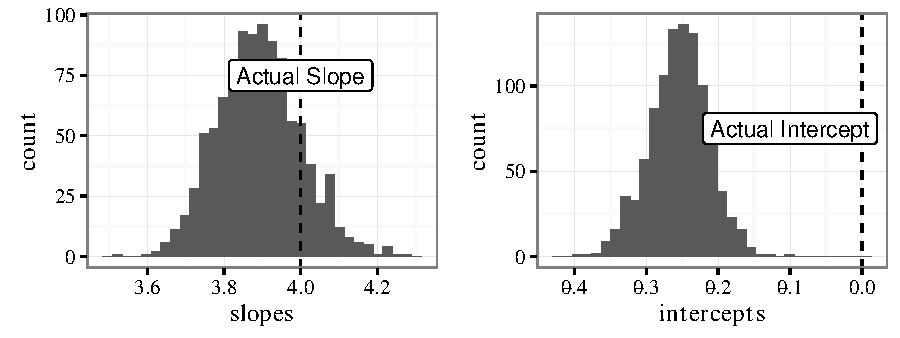
\includegraphics{figure/missing_model1_estimates.pdf}
  \caption[Simulated example of biased estimates from nonignorable missing response]{Simulated example of logistic regression fits to a model with nonignorable
  missing response. One data set of size $n = 10^4$ was computed from the toy data model.
  We then recomputed $R$ 1,000 times, each time fitting a simple logistic regression
  model to $y$ and $X$. \label{fig:missing-model1-estimates}}
  \end{figure}
  
  If we attempt to fit a logistic regression model to this data our
  estimate of the intercept will be inaccurate.
  \autoref{fig:missing-model1-estimates} shows the results of a
  simulation, computing the slope and intercepts for 1,000 different
  patterns of missing data for the same generated data set generated from
  our toy data model.
  
  It makes sense that we are underestimating our intercept. The intercept
  can be interpreted as the base rate, and if values of \(y_i = 1\) are
  more likely to be missing, the overall rate we observe will be lower.
  
  Clearly, if we have nonignorable missing response, we are in a bad
  situation. Having missingness depend on \(Y\) leads to biased estimates
  of our intercepts when we fit models. But we do have all of our
  predictors of \(y\), with no missingness. Could we leverage our
  understanding of how \(X\) predicts \(Y\) to understand the patterns of
  missing response?
  
  \section{Modeling the Missing Data Mechanism with Expectation
  Maximization}\label{em-algorithm}
  
  Here we perform the expectation maximization (EM) algorithm using the
  weighting method proposed by Ibrahim and Lipsitz\footnote{Ibrahim \&
    Lipsitz (1996)}. Let \(y\) be our binary response and \(X\) be our
  predictors. With these we have our complete data logistic regression
  model \(f(y \;|\; X, \beta)\), where \(\beta\) is a vector of parameters
  in the complete data model.
  
  We then specify a logistic regression model for missingness (\(R\)):
  \(f(R \;|\; X, y, \alpha)\), where \(\alpha\) is the vector of
  parameters in the missingness model.
  
  We begin the algorithm by getting our first estimates of \(\alpha\) and
  \(\beta\). We obtain \(\beta^{(1)}\) by estimating \(\beta\) with only
  the non-missing data (\emph{i.e.} fit the models as if there were no
  missing data). We can then estimate \(y\) for the missing data using
  \(\beta^{(1)}\), and then use those estimates to compute
  \(\alpha^{(1)}\).
  
  For the E-step, we compute weights for each observation with missing
  response, representing the probability that the \(i\)th observation has
  response value \(y_i\):
  
  \begin{equation}
  w_{i\: y_i}^{(t)} = 
  f(y_i \;|\; r_i, x_i, \alpha^{(t)}, \beta^{(t)}) =
  \frac{f(y_i \;|\; x_i, \beta^{(t)}) f(r_i \;|\; x_i, y_i, \alpha^{(t)})}{
  \sum_{y_i \in \{0,1\}}
  f(y_i \;|\; x_i, \beta^{(t)}) f(r_i \;|\; x_i, y_i, \alpha^{(t)})
  }.
  \label{eq:weights}
  \end{equation}
  
  \ref{eq:weights} is essentially an application of Bayes' theorem. We can
  view \(f(y_i \;|\; r_i, x_i, \alpha^{(t)}, \beta^{(t)})\) as the
  posterior density of \(y_i\) given observation \(i\) is missing, where
  \(f(y_i \;|\; x_i, \beta^{(t)})\) is the prior distribution and
  \(f(r_i \;|\; x_i, y_i, \alpha^{(t)})\) serves as the likelihood.
  
  For observed responses, \(w_{i\: y_i}^{(t)} = 1\). Note that for each
  observation \(i\), \(\sum_{y_i \in \{0,1\}} w_{i\; y_i} = 1.\) We can
  compute \(f(y_i \;|\; x_i, \beta^{(t)})\) and
  \(f(r_i \;|\; x_i, y_i, \alpha^{(t)})\) by making use of predictions
  from regression models. So in \texttt{R}, we can fit models and use the
  \texttt{predict()} function to get our probabilities from each of these
  models.
  
  For the M-step, we find our next estimates of the parameters,
  \(\alpha^{(t + 1)}\) and \(\beta^{(t + 1)}\), by maximizing
  
  \begin{equation}
  Q(\alpha, \beta \;|\; \alpha^{(t)}, \beta^{(t)}) =
  \sum_{i = 1}^n \sum_{y_i \in \{0,1\}} w_{iy_i}^{(t)} \cdot 
  l(\alpha, \beta | x_i, y_i, r_i).
  \end{equation}
  
  We do this by first by estimating \(\beta^{(t + 1)}\) using weighted
  maximum likelihood for the complete data model, and then estimating
  \(\alpha^{(t + 1)}\) using the same method. To maximize
  \(l(\alpha, \beta | x_i, y_i, r_i)\), we maximize the product of their
  likelihoods,
  \[l(\alpha, \beta | x_i, y_i, r_i) = l(\beta | x_i, y_i) l(\alpha | r_i, x_i, y_i),\]
  which we can maximize by maximizing each of the likelihoods separately
  because our estimates of \(\alpha\) and \(\beta\) are only dependent on
  each other through \(x\) and \(y\). This allows us to use any package
  that can fit models by maximum likelihood estimation using weights for
  the observations, which includes all of the model fitting packages we
  used in Chapter 3.
  
  In order to create the data to fit these models, we create an augmented
  data set where each observation missing the response is recorded as two
  rows. These duplicate rows represent the two possible values of the
  response, and also contain the weights computed in the E-step.
  \autoref{fig:augmented-data} describes this process graphically.
  
  \begin{figure}[htb]
  \centering
  \caption[How to create augmented data for EM algorithm]{
  How to create augmented data for EM algorithm: duplicate rows that are missing
  the response variable, assigning to each row a possible value of the reponse
  and its associated weight. \label{fig:augmented-data}}
  \begin{tabular}{lcl}
  \toprule
  \textbf{Original Data} &  & \textbf{Augmented Data}\\
  \midrule
  
  \begin{tabular}{lll}
  $y_i$ & $x_i$ & $r_i$\\
  \midrule
  1 & 2.4 & 0\\
  0 & 1.3 & 0\\
  NA & -0.4 & 0\\
  & &
  \end{tabular}
  &
  $\to$
  &
  \begin{tabular}{llll}
  $y_i$ & $x_i$ & $r_i$ & $w_i$\\
  \midrule
  1 & 2.4 & 0 & 1\\
  0 & 1.3 & 0 & 1\\
  1 & -0.4 & 0 & 0.2\\
  0 & -0.4 & 0 & 0.8
  \end{tabular}\\
  \bottomrule
  \end{tabular}
  \end{figure}
  
  We repeat the E and M step until the joint loglikelihood converges to
  within some tolerance. An implementation of this algorithm can be found
  in \autoref{em-implementation}.
  
  As an example, we simulated a dataset from the same model we presented
  earlier of size \(10^4\). Of those observations, 6,252 were missing. As
  shown in \autoref{tab:EM-sim}, the estimate for the intercept in the
  model that only considers the complete data is way off, but the model
  resulting from the EM algorithm is nearly as accurate as the model fit
  to the full data (with missing values filled in from the original data
  model.) The missing data model is also able to get accurate estimates of
  the parameters that define the missing data mechanism, but the estimates
  are quite uncertain.
  
  \begin{table}[htb]
  \caption{Coefficients for models fit to simulated data set ($\pm$ twice the
  standard error.) \label{tab:EM-sim}}
  \centering
  \begin{tabular}{lrrrr}
  \toprule
  Model & $\hat{\beta}_0$ & $2 \cdot SE_{\hat{\beta}_0}$  & 
  $\hat{\beta}_X$ &  $2 \cdot SE_{\hat{\beta}_X}$\\
  \midrule
  Actual & 0 & -- & 4 & --\\
  Full Data Model & $-0.009$ &  $0.065$ & $3.881$ &  $0.080$\\
  Complete Data Model & $-0.278$ & $0.106$ & $3.819$ &  $0.259$\\
  EM Final Model & $0.042$ & $0.065$ & $3.814$ &  $0.157$\\
  \bottomrule
  \end{tabular}
  \end{table}
  
  \begin{table}[htb]
  \caption{Estimates for missing data mechanism for simulated model. \label{tab:EM-sim-missing}}
  \centering
  \begin{tabular}{lrrrr}
  \toprule
  Model & $\hat{\alpha}_0$ & $2 \cdot SE_{\hat{\alpha}_0}$ 
  & $\hat{\alpha}_Y$ &  $2 \cdot SE_{\hat{\alpha}_Y}$\\
  \midrule
  Actual & 0.3 & -- & 0.4 & --\\
  EM Missing Data Model & $0.263$ & $0.132$ & $0.530$ &  $0.268$\\
  \bottomrule
  \end{tabular}
  \end{table}
  
  \section{EM Algorithm for the Ride
  Data}\label{em-algorithm-for-the-ride-data}
  
  In order to perform the algorithm, we need to specify a model for
  nonresponse. We will use the same predictors that we do in Model 4 for
  ride rating---including a smoothing spline for time of day for weekdays
  and weekends---except we do not use random rider intercepts. For the EM
  algorithm, we use Model 4 as our ride rating model and use the following
  model for the rating nonresponse mechanism:
  
  \begin{equation}
  r_i \sim \text{Bernoulli}(\text{logit}^{-1} (\alpha_0 + y_i \alpha_y + 
  X_i \alpha_x + X^\text{weekend} \cdot f^\text{time.w} (t_i) +
  (1 - X^\text{weekend}) \cdot f^\text{time} (t_i))).
  \end{equation}
  
  \begin{table}[htb]
  \centering
  \caption{Fit summaries for Model 4 and the EM Model\label{tab:em-modelfits}}
  \begin{tabular}{lm{4in}rrr}
  \toprule
  \textbf{Model} & \textbf{Separation Plot} & \textbf{AUC}\footnotemark\\
  \midrule
  Model 4 & 
\includegraphics{figure/model4-sep.pdf}
  & 0.802\\
  EM Model & 
\includegraphics{figure/em-separation-plot.pdf}
  & 0.763\\
  \bottomrule
  \end{tabular}
  \end{table}
  
  The fit for the EM algorithm seems to be worse. The AUC, shown in
  \autoref{tab:em-modelfits}, which was computed on the complete data, was
  lower than that of Model 4.
  
  \begin{table}[htb]
  \caption{Ride rating model estimates after EM algorithm \label{tab:em-model-estimates}}
  \centering
  \begin{tabular}{lrrrr}
  \toprule
  \textbf{Parameter} & \textbf{Model 4} & \textbf{EM Model}\\
  \midrule
  Log(Length) & -0.147 & 0.205\\
  & \footnotesize (-0.290, -0.005) & \footnotesize (0.106, 0.304)\\
  Mean Temperature & 0.142 & 0.100\\
  & \footnotesize (0.004, 0.281) & \footnotesize (0.005, 0.196)\\
  Mean Wind Speed & 0.002 & -0.026\\
  & \footnotesize (-0.054, 0.057) & \footnotesize (-0.069, 0.016)\\
  Max Gust Speed & -0.005 & 0.020\\
  & \footnotesize (-0.031, 0.021) & \footnotesize (0.001, 0.039)\\
  Rainfall & 0.050 & 0.051\\
  & \footnotesize (-0.017, 0.117) & \footnotesize (0.009, 0.093)\\
  Rainfall 4-Hour & 0.022 & 0.017\\
  & \footnotesize (0.003, 0.041) & \footnotesize (0.003, 0.030)\\
  Intercept & -2.792 & -3.144\\
  & \footnotesize (-3.334, -2.250) & \footnotesize (-3.604, -2.684)\\
  \bottomrule
  \end{tabular}
  \end{table}
  
  There are two disagreements between the EM model and Model 4 for ride
  rating: the coefficients for \(x^\text{length}\) and \(x^\text{rain}\).
  The former has flipped sign while the latter has much less uncertainty
  in its estimate.
  
  The coefficients for the missing model, shown in
  \autoref{tab:nonresponse-estimates} confirm our worry that many of the
  rides missing the rating are not bike rides. These model coefficients
  suggests that rides are much more likely to be missing if they have a
  negative rating. We hypothesized that there would be a weak negative
  effect of a negative rating on missingness; while any reasonable
  researcher wouldn't dismiss the estimates because the sign wasn't what
  was expected, the magnitude seems much more in line with the hypothesis
  that many of the missing ratings correspond to car rides.
  
  It's tempting to suggest that longer rides tend to be missing, but they
  are also more likely to be rated negatively; the distribution of ride
  lengths are actually about the same for rated and non-rated rides. But
  does it make sense that we would have the same distribution of ride
  lengths for rated and non-rated rides, if we suspect many of the
  non-rated rides are actually car rides? Yes, so long as we keep in mind
  that these are rides that have been misclassified as bike rides; we
  expect the classifier already filtered out car rides that were too long
  and fast to be bike rides.
  
  \begin{table}[htb]
  \caption[Estimates for ride rating nonresponse mechanism]{
  Estimates for ride rating nonresponse mechanism. The Basic Nonresponse
  Model is estimated based on the data with $y$ predicted by Model 4. The EM 
  Nonresponse Model is estimated with the EM algorithm, which uses the same
  model specifications. \label{tab:nonresponse-estimates}}
  \centering
  \begin{tabular}{lrrrr}
  \toprule
  \textbf{Parameter} & \textbf{Basic Nonresponse Model} & \textbf{EM Nonresponse Model}\\
  \midrule
  $y$ & 0.730 & 1.035\\
  & \footnotesize (0.235, 1.224) & \footnotesize (0.493, 1.577) \\
  Log(Length) & -0.297 & -0.327\\
  & \footnotesize (-0.362, -0.232) & \footnotesize (-0.393, -0.262)\\
  Mean Temperature & 0.200 & 0.139\\
  & \footnotesize (0.139, 0.262) & \footnotesize (0.077, -0.262)\\
  Mean Wind Speed & 0.032 & 0.031\\
  & \footnotesize (0.003, 0.060) & \footnotesize (0.001, 0.061) \\
  Max Gust Speed & -0.003 & -0.007\\
  & \footnotesize (-0.016, 0.010) & \footnotesize (-0.021, 0.006) \\
  Rainfall & 0.007 & -0.024\\
  & \footnotesize (-0.028, 0.041) & \footnotesize (-0.057, 0.009)\\
  Rainfall 4-Hour & -0.002 & 0.010\\
  & \footnotesize (-0.012, 0.009) & \footnotesize (-0.001, 0.021) \\
  Intercept & -0.927 & -0.967\\
  & \footnotesize (-1.124, -0.729) & \footnotesize (-1.163, -0.771)\\
  \bottomrule
  \end{tabular}
  \end{table}
  
  Unfortunately, these models do not seem ready for use on the \emph{Ride
  Report} data until the quality of data with missing ratings can be
  assured. Knock Software is planning on fixing this, so such an analysis
  may be viable within a year or two of collecting new data. (Because the
  accelorometer data is not saved, they cannot go back and attempt to
  reclassify old rides.)
  
  \chapter{Unfinished Work: Incorporating Routes}\label{routes}
  
  These models so far do not incorporate routes. Though our initial aim
  was to create models that use the routes, we were not able to transform
  the route to a state that was useful for modeling. I leave the models as
  they are, but here I explain some of my work toward the goal of
  incorporating routes and describe some potential modeling approaches.
  Throughout this work is the caveat that many of these results are hard
  to interpret without taking into account route. We hope future
  researchers will be able to accomplish this.
  
  \section{Data Structures for Routes}\label{data-structures-for-routes}
  
  Before one can model routes, they need to be represented properly. Ride
  Report's approach has been to discretize the routes into road segments
  by map matching the GPS traces to road segments in the Open Street Map
  (OSM) data. Road segments are readily availible in the OSM data sets as
  well as in shapefiles published by cities. In particular, Civicapps.org,
  a public data portal for the Portland, OR area has a shapefile of the
  bicycle network in Portland, OR, with information about the type of
  roads, presence of bike lanes, and other useful information about the
  roads bikes have access to in Portland.
  
  Road segments are not the only way to represent routes, however. One
  could also consider a route as a sequence of intersections or
  intersections and road segments. Though modeling intersections may be
  more difficult, it's likely they could be more interesting parts of the
  routes. In the bike accident data examined by Meyers, most of the
  accidents occurred at intersections\footnote{Meyers (2015)}, so it would
  make sense if these were often the most stressful and dangerous portion
  of riders' routes.
  
  For now, however, the most readily available data are on road segments.
  
  \section{Regression Terms for Road
  Segments}\label{regression-terms-for-road-segments}
  
  How could we use our knowledge of riders' routes into our regression?
  The approach we present here will be to consider routes as sequences of
  discrete road segments, each of which have known properties. As
  mentioned before, there are data about roads that give information about
  bike lanes, road size, and other attributes of road segments.
  
  Ideally we would like to estimate some parameter for each road segment
  that indicated its typical contribution to the probability of a negative
  ride rating. The most immediate hurdle is figuring out how to estimate
  all of those parameters, particularly when the number of rides per a
  particular road segment may be low.
  
  Bayesian inference may be the best bet to get something for each road
  segment, but as a extremely simple example, we outline here a method
  that would be easy to fit, but likely not a very good model. Regardless,
  it gives a good idea of how the ideas of multilevel models could be
  adapted for use with road segments, despite the lack of a clear
  hierarchy. Assume we have \(K\) total road segments in our road network
  and for each ride we have \(\Omega_i \subseteq \{1, \ldots, K\}\), the
  set of road segments that are in the route of ride \(i\). Let \(l_k\) be
  the length of the \(k\)th segment and define the length of ride \(i\) to
  be:
  
  \[ L_i = \sum_{k \in \Omega_i} l_k.\]
  
  For the \(k\)th road segment, define the \(m\)-dimensional vector
  \(W_k = W_k^1, W_k^2, \ldots, W_k^m\) road segment-level predictors.
  Then we shall define the term in our regression for the route of ride
  \(i\) as
  
  \[ R_i = \frac{1}{L_i} \sum_{k \in \Omega_i} l_k W_k \beta^{\text{road}},\]
  
  Where \(\beta^{\text{road}}\) is a vector of coefficients for the road
  segment level predictors. When actually computing this value, we can
  factor out the \(\beta^{\text{road}}\), and then the rest of \(R_i\) is
  just a transformation of road-level variables.
  
  \chapter*{Conclusion}\label{conclusion}
  \addcontentsline{toc}{chapter}{Conclusion}
  
  \setcounter{chapter}{7} \setcounter{section}{0}
  
  By focusing on minimizing barriers to responding and automating as much
  of the data collection as possible, the designers of the \emph{Ride
  Report} app created an infrastructure that could collect large numbers
  of ride ratings. But sample size isn't everything: the subjectivity of
  the ratings and the pattern of missing ratings make this a treacherous
  data set to model naively.
  
  The subjective ratings pose a problem particularly when used to infer
  the quality of particular road segments; if most of the rides are by one
  particular rider, then the typical rating over that segment will reflect
  that particular rider's interpretation of the ratings more than others.
  Our models from \autoref{model-chapter} confirm that modeling ride
  rating with rider intercepts is essential. Adding rider intercepts to a
  multivariate regression model increased the cross-validated AUC from
  0.552---little better than the null model---to 0.797. These intercepts
  turned out to encode much more than a rider's baseline tendency to rate
  a ride negatively; \autoref{fig:time-pred-plot} showed how much
  information rider intercepts had about riders' typical time of day, and
  it's likely that riders' typical routes are also encoded in these
  intercepts as well. Future research should pay special attention to how
  these intercepts change when routes are incorporated into these models.
  
  Our missing data models showed some questionable results, though it's
  hard to know if those issues stem from the data quality of the unrated
  rides or a flaw in the model. If many of the unrated rides are actually
  not bicycle rides--- which we suspect is the case---then these missing
  data models will not be appropriate until the misclassification of
  non-bike rides as bike rides is no longer a problem.
  
  In some ways, this is an incomplete work. To leverage the insights from
  this paper in creating a map of good and bad routes, models that use
  ride route information need to be developed and implemented. Both the
  theoretical development and the technical implementation are difficult
  problems in and of themselves. There are many ways one could model the
  relationship between ride rating and route, and it's difficult to find
  any good theoretical justification for one particular model. And even if
  a good theoretical model can be formulated, such models will likely not
  be simple to implement, both because the models will probably not be
  supported by common model fitting packages and because matching the GPS
  traces to the road network model is a difficult inference problem in
  itself.
  
  \appendix
  
  \chapter{A Code Sample of the EM Algorithm}\label{em-implementation}
  
  Despite its attractive features, there are few explicit explanation of
  how to actually program the EM algorithm for missing response using
  weights. The theoretical is contained in \autoref{em-algorithm}, but for
  the benefit of the reader, we lay out the practical implementation here.
  
  For this example, we present the same code used for the simulation in
  \autoref{em-algorithm}. The data can be simulated with,
  
  \begin{Shaded}
  \begin{Highlighting}[]
  \NormalTok{inv_logit <-}\StringTok{ }\NormalTok{function(x) }\DecValTok{1} \NormalTok{/}\StringTok{ }\NormalTok{(}\DecValTok{1} \NormalTok{+}\StringTok{ }\KeywordTok{exp}\NormalTok{(-x))}
  \NormalTok{n <-}\StringTok{ }\FloatTok{1e3}
  \NormalTok{x <-}\StringTok{ }\KeywordTok{rnorm}\NormalTok{(n, }\DecValTok{0}\NormalTok{, }\DecValTok{1}\NormalTok{)}
  \NormalTok{y <-}\StringTok{ }\KeywordTok{rbinom}\NormalTok{(n, }\DecValTok{1}\NormalTok{, }\DataTypeTok{prob =} \KeywordTok{inv_logit}\NormalTok{(}\DecValTok{4} \NormalTok{*}\StringTok{ }\NormalTok{x))}
  \NormalTok{r <-}\StringTok{ }\KeywordTok{rbinom}\NormalTok{(n, }\DecValTok{1}\NormalTok{, }\DataTypeTok{prob =} \KeywordTok{inv_logit}\NormalTok{(}\FloatTok{0.3} \NormalTok{+}\StringTok{ }\FloatTok{0.4} \NormalTok{*}\StringTok{ }\NormalTok{y))}
  
  \NormalTok{simulated_data <-}\StringTok{ }\KeywordTok{data.frame}\NormalTok{(x, y, r)}
  \NormalTok{simulated_data$y <-}\StringTok{ }\KeywordTok{ifelse}\NormalTok{(simulated_data$r ==}\StringTok{ }\DecValTok{1}\NormalTok{, }\OtherTok{NA}\NormalTok{, simulated_data$y)}
  \end{Highlighting}
  \end{Shaded}
  
  For convenience, we define the models once as functions, so we can use
  them more than once.
  
  \begin{Shaded}
  \begin{Highlighting}[]
  \NormalTok{fit_r <-}\StringTok{ }\NormalTok{function(data, }\DataTypeTok{weights =} \OtherTok{NULL}\NormalTok{) \{}
    \KeywordTok{gam}\NormalTok{(r ~}\StringTok{ }\NormalTok{x +}\StringTok{ }\NormalTok{y_pred, }\DataTypeTok{data =} \NormalTok{data, }\DataTypeTok{family =} \NormalTok{binomial, }\DataTypeTok{weights =} \NormalTok{weights)}
  \NormalTok{\}}
  \NormalTok{fit_y <-}\StringTok{ }\NormalTok{function(data, }\DataTypeTok{weights =} \OtherTok{NULL}\NormalTok{) \{}
    \KeywordTok{gam}\NormalTok{(y_pred ~}\StringTok{ }\NormalTok{x, }\DataTypeTok{data =} \NormalTok{data, }\DataTypeTok{family =} \NormalTok{binomial, }\DataTypeTok{weights =} \NormalTok{weights)}
  \NormalTok{\}}
  \end{Highlighting}
  \end{Shaded}
  
  First, we separate out the portions of the data that are complete and
  that are missing the response. To make our code clear and simple, we
  make use of the \texttt{dplyr} package.
  
  \begin{Shaded}
  \begin{Highlighting}[]
  \NormalTok{data_complete <-}\StringTok{ }\NormalTok{simulated_data %>%}\StringTok{ }\KeywordTok{filter}\NormalTok{(!}\KeywordTok{is.na}\NormalTok{(y)) %>%}\StringTok{ }\KeywordTok{mutate}\NormalTok{(}\DataTypeTok{weight =} \DecValTok{1}\NormalTok{)}
  \NormalTok{data_missing <-}\StringTok{ }\NormalTok{simulated_data %>%}\StringTok{ }\KeywordTok{filter}\NormalTok{(}\KeywordTok{is.na}\NormalTok{(y)) %>%}\StringTok{ }\KeywordTok{mutate}\NormalTok{(}\DataTypeTok{weight =} \OtherTok{NA}\NormalTok{)}
  \end{Highlighting}
  \end{Shaded}
  
  We then start the algorithm with our initial guesses at the model for
  \texttt{y} and \texttt{r}:
  
  \begin{Shaded}
  \begin{Highlighting}[]
  \NormalTok{simulated_data$y_pred <-}\StringTok{ }\NormalTok{simulated_data$y}
  \NormalTok{model_y <-}\StringTok{ }\KeywordTok{fit_model_y}\NormalTok{(data_complete)}
  \NormalTok{simulated_data$y_pred <-}\StringTok{ }\NormalTok{(}\KeywordTok{predict}\NormalTok{(model_y,}
                                    \DataTypeTok{newdata =} \NormalTok{simulated_data,}
                                    \DataTypeTok{type =} \StringTok{"response"}\NormalTok{) >}\StringTok{ }\FloatTok{0.5}\NormalTok{) %>%}\StringTok{ }\KeywordTok{as.numeric}\NormalTok{()}
  \NormalTok{model_r <-}\StringTok{ }\KeywordTok{fit_model_r}\NormalTok{(simulated_data)}
  \end{Highlighting}
  \end{Shaded}
  
  Finally, we perform the main loop of EM algorithm iterations. We have
  two stopping conditions here: when the algorithm reaches the maximum
  number of iterations or when the difference between the current model's
  AIC and the previous model's AIC is less than the tolerance.
  
  \begin{Shaded}
  \begin{Highlighting}[]
  \NormalTok{last_aic <-}\StringTok{ }\KeywordTok{AIC}\NormalTok{(model_y)}
  
  \NormalTok{for (i in }\DecValTok{1}\NormalTok{:}\DecValTok{1000}\NormalTok{) \{}
    \CommentTok{# get prob of 1}
    \NormalTok{y_pred <-}\StringTok{ }\KeywordTok{predict}\NormalTok{(model_y, }\DataTypeTok{newdata =} \NormalTok{data_missing, }\DataTypeTok{type=}\StringTok{"response"}\NormalTok{)}
    
    \CommentTok{# get prob missing given y}
    \NormalTok{pred_r_y1 <-}\StringTok{ }\KeywordTok{predict}\NormalTok{(model_r, }
                         \DataTypeTok{newdata =} \KeywordTok{mutate}\NormalTok{(data_missing, }\DataTypeTok{y_pred =} \DecValTok{1}\NormalTok{), }
                         \DataTypeTok{type=}\StringTok{"response"}\NormalTok{)}
    \NormalTok{pred_r_y0 <-}\StringTok{ }\KeywordTok{predict}\NormalTok{(model_r, }
                         \DataTypeTok{newdata =} \KeywordTok{mutate}\NormalTok{(data_missing, }\DataTypeTok{y_pred =} \DecValTok{0}\NormalTok{),}
                         \DataTypeTok{type=}\StringTok{"response"}\NormalTok{)}
    
    \CommentTok{# Make weights}
    \NormalTok{denom <-}\StringTok{ }\NormalTok{(y_pred *}\StringTok{ }\NormalTok{pred_r_y1) +}\StringTok{ }\NormalTok{((}\DecValTok{1}\NormalTok{-y_pred) *}\StringTok{ }\NormalTok{pred_r_y0)}
    \NormalTok{w_y1 <-}\StringTok{ }\NormalTok{y_pred *}\StringTok{ }\NormalTok{pred_r_y1 /}\StringTok{ }\NormalTok{denom}
    \NormalTok{w_y2 <-}\StringTok{ }\NormalTok{(}\DecValTok{1}\NormalTok{-y_pred) *}\StringTok{ }\NormalTok{pred_r_y0 /}\StringTok{ }\NormalTok{denom}
    
   \CommentTok{# print(pred)}
    \NormalTok{data_augmented <-}\StringTok{ }\KeywordTok{bind_rows}\NormalTok{(data_complete,}
                          \KeywordTok{mutate}\NormalTok{(data_missing,}
                                 \DataTypeTok{weight =} \NormalTok{w_y1, }
                                 \DataTypeTok{y_pred =} \DecValTok{1}\NormalTok{),}
                          \KeywordTok{mutate}\NormalTok{(data_missing,}
                                 \DataTypeTok{weight =} \NormalTok{w_y2,}
                                 \DataTypeTok{y_pred =} \DecValTok{0}\NormalTok{))}
    \NormalTok{model_y <-}\StringTok{ }\KeywordTok{fit_y}\NormalTok{(data_augmented,}
                           \NormalTok{data_augmented$weight)}
    \NormalTok{model_r <-}\StringTok{ }\KeywordTok{fit_r}\NormalTok{(data_augmented,}
                           \NormalTok{data_augmented$weight)}
    
    \CommentTok{# Check Stopping Condition}
    \NormalTok{current_aic <-}\StringTok{ }\KeywordTok{AIC}\NormalTok{(model_y)}
    \KeywordTok{print}\NormalTok{(}\KeywordTok{AIC}\NormalTok{(model_y))}
    \NormalTok{if ((i >}\StringTok{ }\DecValTok{1}\NormalTok{) &&}\StringTok{ }\NormalTok{(last_aic -}\StringTok{ }\NormalTok{current_aic <}\StringTok{ }\FloatTok{0.0001}\NormalTok{)) break}
    \NormalTok{last_aic <-}\StringTok{ }\NormalTok{current_aic}
  \NormalTok{\}}
  \end{Highlighting}
  \end{Shaded}
  
  \backmatter
  
  \chapter{References}\label{references}
  
  \noindent
  
  \setlength{\parindent}{-0.20in} \setlength{\leftskip}{0.20in}
  \setlength{\parskip}{8pt}
  
  \hypertarget{refs}{}
  \hypertarget{ref-lme4}{}
  Bates, D., Mächler, M., Bolker, B., \& Walker, S. (2015). Fitting linear
  mixed-effects models using lme4. \emph{Journal of Statistical Software},
  \emph{67}(1), 1--48.
  
  \hypertarget{ref-stan}{}
  Carpenter, B., Gelman, A., Hoffman, M., Lee, D., Goodrich, B.,
  Betancourt, M., \ldots{} Riddell, A. (2016). Stan: A probabilistic
  programming language. \emph{Journal of Statistical Software}.
  
  \hypertarget{ref-cressie2011}{}
  Cressie, N., \& Wikle, C. K. (2011). \emph{Statistics for
  spatio-temporal data}. John Wiley \& Sons.
  
  \hypertarget{ref-gelman}{}
  Gelman, A., \& Hill, J. (2006). \emph{Data analysis using regression and
  multilevel/Hierarchical models}. The Edinburgh Building, Cambridge CB2
  8RU, UK: Cambridge University Press, New York.
  
  \hypertarget{ref-greenhill2011}{}
  Greenhill, B., Ward, M. D., \& Sacks, A. (2011). The separation plot: A
  new visual method for evaluating the fit of binary models.
  \emph{American Journal of Political Science}, \emph{55}(4), 991--1002.
  
  \hypertarget{ref-esl}{}
  Hastie, T., Tibshirani, R., \& Friedman, J. (2008). \emph{The elements
  of statistical learning: Data mining, inference, and prediction} (Second
  edition). Springer.
  
  \hypertarget{ref-ibrahim1996}{}
  Ibrahim, J. G., \& Lipsitz, S. R. (1996). Parameter estimation from
  incomplete data in binomial regression when the missing mechanism is
  nonignorable. \emph{Biometrics}, \emph{52}(3), 1071--1078.
  
  \hypertarget{ref-little1987}{}
  Little, R. J., \& Rubin, D. B. (1987). \emph{Statistical analysis with
  missing data}. John Wiley \& Sons.
  
  \hypertarget{ref-mackaronis2013}{}
  Mackaronis, J. E., Strassberg, D. S., Cundiff, J. M., \& Cann, D. J.
  (2013). Beholder and beheld: A multilevel model of perceived sexual
  appeal. \emph{Archives of Sexual Behavior}.
  
  \hypertarget{ref-meyers2015}{}
  Meyers, R. (2015). Retrieved from
  \url{https://github.com/ReedCollegeMATH241/MATH241_PortlandBikeWorks}
  
  \hypertarget{ref-pdxrain}{}
  Portland Bureau of Environmental Science, C. of. (2016, February).
  Portland fire bureau rain gage data table. Retrieved from
  \url{http://or.water.usgs.gov/non-usgs/bes/ankeny.rain}
  
  \hypertarget{ref-cosmaadditive}{}
  Shalizi, C. (2013a, February). Additive models. Retrieved from
  \url{http://www.stat.cmu.edu/~cshalizi/uADA/13/lectures/ch09.pdf}
  
  \hypertarget{ref-cosmasplines}{}
  Shalizi, C. (2013b, February). Splines. Retrieved from
  \url{http://www.stat.cmu.edu/~cshalizi/uADA/13/lectures/ch08.pdf}
  
  \hypertarget{ref-Rlang}{}
  Team, R. C. (2015). \emph{R: A language and environment for statistical
  computing}. Vienna, Austria: R Foundation for Statistical Computing.
  Retrieved from \url{https://www.R-project.org/}
  
  \hypertarget{ref-gelman2013}{}
  \emph{The garden of forking paths: Why multiple comparisons can be a
  problem, even when there is no ``fishing expedition'' or ``p-hacking''
  and the research hypothesis was posited ahead of time}. (2013, Nov).
  Retrieved from
  \url{http://www.stat.columbia.edu/~gelman/research/unpublished/p_hacking.pdf}
  
  \hypertarget{ref-wunderground}{}
  Weather Underground, I. (2016, February). Weather history for kPDX.
  Retrieved from
  \url{https://www.wunderground.com/history/airport/KPDX/2015/9/20/CustomHistory.html?dayend=8\&monthend=2\&yearend=2016\&req_city=\&req_state=\&req_statename=\&reqdb.zip=\&reqdb.magic=\&reqdb.wmo=\&MR=1}
  
  \hypertarget{ref-wood2006}{}
  Wood, S. (2006). \emph{Generalized additive models: An introduction with
  r}. CRC press.
  
  \hypertarget{ref-gamm4}{}
  Wood, S., \& Scheipl, F. (2014). Gamm4: Generalized additive mixed
  models using mgcv and lme4. Retrieved from
  \url{https://CRAN.R-project.org/package=gamm4}
  
  \hypertarget{ref-ying2006}{}
  Ying, Y., Feinberg, F., \& Wedel, M. (2006). Leveraging missing ratings
  to improve online recommendation systems. \emph{Journal of Marketing
  Research}, \emph{43}(3), 355--365.


  % Index?

\end{document}

